\documentclass[sigconf,edbt]{acmart-edbt2021}

\def\BibTeX{{\rm B\kern-.05em{\sc i\kern-.025em b}\kern-.08em
    T\kern-.1667em\lower.7ex\hbox{E}\kern-.125emX}}

\usepackage{booktabs} % For formal tables
\usepackage{tikz}
\usepackage[noend]{algpseudocode}
\usepackage{algorithm}
\usepackage{algorithmicx}
\usepackage{xcolor}
\usepackage{subcaption}
\usepackage{listings}
\usepackage{extarrows}
\usetikzlibrary{fit,automata,positioning}
\usetikzlibrary{decorations.pathmorphing}
\tikzset{snake it/.style={decorate, decoration=snake}}

\definecolor{lightgray}{gray}{0.9}

% Copyright
\setcopyright{rightsretained}

% DOI
\acmDOI{}

% ISBN
\acmISBN{XXXXXXXX}

%Conference
\acmConference[EDBT 2021]{24th International Conference on Extending Database Technology (EDBT)}{March 23-26, 2021}{Nicosia, Cyprus} 
\acmYear{2021}

\settopmatter{printacmref=false, printccs=false, printfolios=false}

\pagestyle{empty} % removes running headers

% Math square brackets
\DeclareMathOperator{\rank}{rank}
\makeatletter
\newenvironment{sqcases}{%
  \matrix@check\sqcases\env@sqcases
}{%
  \endarray\right.%
}
\def\env@sqcases{%
  \let\@ifnextchar\new@ifnextchar
  \left\lbrack
  \def\arraystretch{1.2}%
  \array{@{}l@{\quad}l@{}}%
}
\makeatother

% Footnote reference
\makeatletter
\newcommand\footnoteref[1]{\protected@xdef\@thefnmark{\ref{#1}}\@footnotemark}
\makeatother

\begin{document}
\title{ContextFree Wars: The RedisGraph Strikes Back}
% \begin{document}
% \title{Implementing support for context-free path queering for the Cypher extension in RedisGraph}
% \titlenote{Produces the permission block, and copyright information}
% \subtitle{Extended Abstract}
% \subtitlenote{The full version of the author's guide is available as
%   \texttt{acmart.pdf} document}
  


\author{Arseniy Terekhov}
	\email{simpletondl@yandex.ru}
	\affiliation{%
		\institution{Saint Petersburg State University}
		\streetaddress{7/9 Universitetskaya nab.}
		\city{St. Petersburg}
		\country{Russia}
		\postcode{199034}
	}

\author{Vlada Pogozhelskaya}
	\email{pogozhelskaya@gmail.com}
	\affiliation{%
		\institution{Saint Petersburg State University}
		\streetaddress{7/9 Universitetskaya nab.}
		\city{St. Petersburg}
		\country{Russia}
		\postcode{199034}
	}

\author{Vadim Abzalov}
	\email{vadim.i.abzalov@gmail.com}
	\affiliation{%
		\institution{Saint Petersburg State University}
		\streetaddress{7/9 Universitetskaya nab.}
		\city{St. Petersburg}
		\country{Russia}
		\postcode{199034}
	}

\author{Timur Zinnatulin}
	\email{!!!@!!!}
	\affiliation{%
		\institution{Saint Petersburg State University}
		\streetaddress{7/9 Universitetskaya nab.}
		\city{St. Petersburg}
		\country{Russia}
		\postcode{199034}
	}	

\author{Semyon Grigorev}
	\email{s.v.grigoriev@spbu.ru}
	\email{semyon.grigorev@jetbrains.com}
	\orcid{0000-0002-7966-0698}
	\affiliation{
		\institution{Saint Petersburg State University}
		\streetaddress{7/9 Universitetskaya nab.}
		\city{St. Petersburg}
		\country{Russia}
		\postcode{199034}
	}
	\affiliation{
		\institution{JetBrains Research}
		\streetaddress{Primorskiy prospekt 68-70, Building 1}
		\city{St. Petersburg}
		\country{Russia}
		\postcode{199034}
	}

% The default list of authors is too long for headers}
% \renewcommand{\shortauthors}{B. Trovato et al.}
\renewcommand{\shortauthors}{Arseniy Terekhov et al.}


\begin{abstract}
A long time ago in a galaxy far far away...
Abstract is very abstract. Abstract is very abstract. Abstract is very abstract. Abstract is very abstract. Abstract is very abstract. Abstract is very abstract. Abstract is very abstract. Abstract is very abstract. Abstract is very abstract. Abstract is very abstract. Abstract is very abstract. Abstract is very abstract. Abstract is very abstract. Abstract is very abstract. Abstract is very abstract. Abstract is very abstract. Abstract is very abstract. Abstract is very abstract. Abstract is very abstract. Abstract is very abstract. Abstract is very abstract. Abstract is very abstract. 
\end{abstract}

%
% % The code below should be generated by the tool at
% % http://dl.acm.org/ccs.cfm
% % Please copy and paste the code instead of the example below. 
% %
\begin{CCSXML}
		<ccs2012>
		<concept>
			<concept_id>10002951.10002952.10003197.10010825</concept_id>
			<concept_desc>Information systems~Query languages for non-relational engines</concept_desc>
			<concept_significance>500</concept_significance>
		</concept>
		<concept>
			<concept_id>10003752.10003766.10003771</concept_id>
			<concept_desc>Theory of computation~Grammars and context-free languages</concept_desc>
			<concept_significance>500</concept_significance>
		</concept>
		<concept>
			<concept_id>10002950.10003624.10003633.10003640</concept_id>
			<concept_desc>Mathematics of computing~Paths and connectivity problems</concept_desc>
			<concept_significance>300</concept_significance>
		</concept>
		<concept>
			<concept_id>10002951.10002952.10002953.10010146</concept_id>
			<concept_desc>Information systems~Graph-based database models</concept_desc>
			<concept_significance>500</concept_significance>
		</concept>
		</ccs2012>
\end{CCSXML}
	
    \ccsdesc[500]{Information systems~Graph-based database models}
	\ccsdesc[500]{Information systems~Query languages for non-relational engines}
	\ccsdesc[500]{Theory of computation~Grammars and context-free languages}
    \ccsdesc[300]{Mathematics of computing~Paths and connectivity problems}


% \keywords{ACM proceedings, \LaTeX, text tagging}

%% A "teaser" image appears between the author and affiliation
%% information and the body of the document, and typically spans the
%% page.
%\begin{teaserfigure}
%  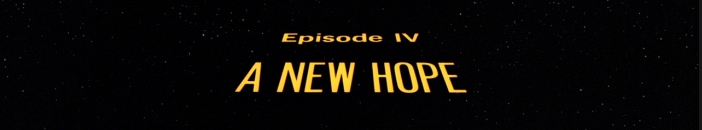
\includegraphics[width=\textwidth]{new_hope.png}
%  \caption{Episode IV: A New Hope}
%  \label{fig:teaser}
%\end{teaserfigure}

\maketitle

\chapter*{Введение}                         % Заголовок
\addcontentsline{toc}{chapter}{Введение}    % Добавляем его в оглавление
\textbf{Актуальность работы}

Статический анализ исходного кода является известной техникой  получения знаний о программе без её исполнения ~\cite{StaticCodeAnalysis3,StaticCodeAnalysis2,StaticCodeAnalysis1}. Статический анализ является неотъемлемой частью многих процессов, связанных с разработкой программного обеспечения (ПО), и может использоваться, например, для упрощения работы с кодом с помощью подсветки синтаксиса языка в программах, навигации по коду, реализации контекстных подсказок. Более того, статический анализ используется для обнаружения ошибок на ранних стадиях разработки, до запуска программы, а также для поиска различных семантических ошибок, которые не могут быть определены обычным синтаксическим анализом.  Также, статический анализ используется при решении задач трансформации исходного кода и реинжиниринге~\cite{reengANT}. Однако во многих языках программирования имеются конструкции, которые существенно затрудняют статический анализ. 

Например, широко используются динамические встроенные языки --- приложение, созданное на одном языке, генерирует программу на другом языке и передаёт её на выполнение в соответствующее окружение. Примерами могут служить динамические SQL-запросы к базам данных из приложений на Java, С++, С\#, формирование HTML-страниц в PHP-приложениях~\cite{DSQLISO,JSP,PHPmySQL}. Генерируемый код собирается из строк таким образом, чтобы в момент выполнения результирующая строка представляла собой корректную программу. Примеры использования встроенных языков представлены в листингах~\ref{lst:dsql1},~\ref{lst:JsJava} и~\ref{lst:PhPSqlHtml}. Следует отметить, что одна программа может генерировать код на нескольких языках (см. листинг~\ref{lst:PhPSqlHtml}). При этом возможно получение частей кода из разных источников (например, учитывать текстовый ввод пользователя, что часто используется для задания фильтров при конструировании SQL-запросов). Использование динамически формируемых программ  позволяет избежать дополнительных накладных расходов, присущих таким технологиям, как ORM\footnote{ORM или Object-Relational Mapping --- технология программирования, которая связывает базы данных с концепциями объектно-ориентированных языков программирования~\cite{ORM}.}, и достичь высокой производительности. Благодаря этому использование динамически генерируемых программ получило широкое распространение и применяется до сих пор. Вместе с этим, несмотря на появление новых технологий, динамическая генерация SQL-запросов активно используется и в настоящее время~\cite{DSQLInActiveUse}.

\fvset{frame=lines,framesep=5pt,fontsize=\small}\

\begin{listing}
    \begin{pyglist}[language=sql,numbers=left,numbersep=5pt]

CREATE PROCEDURE [dbo].[MyProc]  @TABLERes   VarChar(30)
AS
    EXECUTE ('INSERT INTO ' + @TABLERes + ' (sText1)' +
             ' SELECT ''Additional condition: '' + sName' +
             ' from #tt where sAction = ''1000000''')
GO
    \end{pyglist}
\caption{Код с использованием динамического SQL}
\label{lst:dsql1}
\end{listing} 
 
\fvset{frame=lines,framesep=5pt}
\begin{listing}
    \begin{pyglist}[language=java,numbers=left,numbersep=5pt]
import javax.script.*;  
public class InvokeScriptFunction {  
    public static void main(String[] args) throws Exception {  
        ScriptEngineManager manager = new ScriptEngineManager();  
        ScriptEngine engine = manager.getEngineByName("JavaScript");  
        // JavaScript code in a String  
        String script = 
            "function hello(name) { print('Hello, ' + name); }";  
        // evaluate script  
        engine.eval(script);  
        // javax.script.Invocable is an optional interface.  
        // Check whether your script engine implements or not!  
        // Note that the JavaScript engine implements
        // Invocable interface.  
        Invocable inv = (Invocable) engine;  
        // invoke the global function named "hello"  
        inv.invokeFunction("hello", "Scripting!!" );  
    }  
}
    \end{pyglist}
\caption{Вызов JavaScript из Java}
\label{lst:JsJava}
\end{listing}


\fvset{frame=lines,framesep=5pt}
\begin{listing}
    \begin{pyglist}[language=php,numbers=left,numbersep=5pt]

<?php
    // Embedded SQL
    $query = 'SELECT * FROM ' . $my_table; 
    $result = mysql_query($query);
    
    // HTML markup generation
    echo "<table>\n";
    while ($line = mysql_fetch_array($result, MYSQL_ASSOC)) {
        echo "\t<tr>\n";    
        foreach ($line as $col_value) {
            echo "\t\t<td>$col_value</td>\n";
        }
        echo "\t</tr>\n";
    }
    echo "</table>\n";
?>
    \end{pyglist}
\caption{Использование нескольких встроенных в PHP языков (MySQL, HTML)}
\label{lst:PhPSqlHtml}
\end{listing}



Динамически формируемые выражения часто конструируются с помощью таких операций, как конкатенация в циклах или условных предложениях, или в рекурсивных процедурах. Это затрудняет статический анализ и приводит к получению множества возможных значений для каждого выражения в момент выполнения. Вследствие этого фрагменты динамически формируемого кода воспринимаются компилятором исходного языка как простые строки, не подлежащие дополнительному анализу, а это, в свою очередь, приводит к высокой вероятности возникновения ошибок во время выполнения программы. В худшем случае такая ошибка не приведёт к прекращению работы приложения, что указало бы на проблемы, однако целостность данных при этом может оказаться нарушена. Более того, использование динамически формируемых выражений затрудняет не только разработку информационных систем, так и также и реинжиниринг, поскольку в последнем случае важно автоматизировать перенос системы на новые зыки и платформы, что невозможно без качественного статического анализа. Например, при наличии в коде приложения динамически формируемых SQL-запросов нельзя точно ответить на вопрос о том, с какими элементами базы данных не взаимодействует система, и удалить их. При переносе такой системы на другую СУБД необходимо гарантировать, что для всех динамически формируемых выражений значение в момент выполнения будет корректным кодом на языке новой СУБД~\cite{JSquash}. Следует отметить, что отсутствие статического анализа динамически формируемых программ не позволяет реализовывать для них стандартную функциональность интегрированных сред разработки (Integrated Development Environment, IDE) --- подсветку синтаксиса и автодополнение, рефакторинг кода и т.д. Такая функциональность значительно упрощает процесс разработки и отладки приложений и полезна не только для основного языка, но и для встроенных языков. 

Для решения всех перечисленных выше задач необходимы инструменты, проводящие статический анализ динамически формируемых программ. Такой анализ может дать существенную информацию о таких программах, поскольку редко встречается ситуация полной динамической неопределённости (например, при создании динамических программ исключительно на основе пользовательского ввода). В большинстве случаев, имея программу, генерирующую динамические вставки, с помощью статического анализа можно получить достаточно информации для решения поставленных выше задач. Решению этой проблемы и посвящена данная диссертационная работа. 


\textbf{Степень разработанности темы}

Существуют классические исследования, посвященные разработке компиляторов --- работы А.~Ахо~\cite{Dragon}, А.~Брукера~\cite{CompilerCompiler}, С.~Джонсона~\cite{yaccBook},  Б.К.Мартыненко~\cite{Martinenko1, Martinenko2}  и др.  Однако содержащиеся там алгоритмы синтаксического анализа не могут быть применены к решению задачи анализа динамически формируемых программ, поскольку предназначены для обработки входных данных, представимых в видн линейной последовательности символов, а такое представление динамически формируемых программ не всегда возможно.

Методы обобщённого синтаксического анализа, лежащие в основе данной работы, изложены в трудах таких учёных как Масару Томита (Masaru Tomita)~\cite{Tomita}, Элизабет Скотт (Elizabeth Scott) и Адриан Джонстон (Adrian Johnstone)~\cite{RNGLR,RIGLR} из университета Royal Holloway (Великобритания), Ян Рекерс (Jan Rekers, University of Amsterdam)~\cite{SPPF}, Элко Виссер (Eelco Visser)~\cite{RNGLRSyntaxerror2,RNGLRSyntaxerror3} и других.

Анализу динамически формируемых строковых выражений посвящены работы таких зарубежных учёных как Кюнг-Гу Дох (Kyung-Goo Doh)~\cite{LrAbstract1,LrAbstract2,LRAbstractParsingSema}, Ясухико Минамиде (Minamide Yasuhiko)~\cite{PHPSA}, Андерс Мёллер (Anders M{\o}ller)~\cite{JSA} и отечественных учёных А.А.~Бреслава~\cite{Alvor1,Alvor2} и других. Хорошо изучены вопросы проверки корректности динамически формируемых выражений и поиска фрагментов кода, уязвимых для SQL-инъекций~\cite{SQLInjection,Dasgupta:2009:SAF:1546683.1547548}. Однако данные работы исследуют отдельные аспекты проблемы статического анализа динамически формируемых программ, оставляя в стороне создание готовых алгоритмов (в частности, не строят структурное представление анализируемых программ). В связи с этим возникают проблемы масштабируемости данных результатов, например, создание на их основе более сложных видов статического анализа.

Так же важным является предоставление компонентов, упрощающих создание новых инструментов для решения конкретных задач. Данных подход хорошо исследован в области разработки компиляторов, где широкое распространение получили генераторы анализаторов и пакеты стандартных библиотек (работы А.~Ахо~\cite{Dragon}, А.~Брукера~\cite{CompilerCompiler}, С.~Джонсона~\cite{yaccBook} и др.). 

В работах отечественных учёных М.Д.~Шапот и Э.В.~Попова~\cite{DynamicDSQLTranslation}, а так же зарубежных учёных Антони Клеви (Anthony Cleve), Жан-Люк Эно (Jean-Luc Hainaut)~\cite{DSQLReverseEngineering}, Йост Виссер (Joost Visser)~\cite{DSQLQualityMesure} и других рассматриваются различные аспекты реинжиниринга информационных систем, использующих встроенные SQL-запросы, однако не формулируется общего метода для решения таких задач. Этот вопрос также не затрагивается в классических работах, посвященных реинжиниригу~\cite{SoftwareReeng1, reengANT, SoftwareReeng2, SoftwareReeng3}. Однако разработка такого метода является актуальной задачей.

Таким образом, актуальной является задача дальнейшего исследования статического анализа динамически формируемых строковых выражений. Кроме этого важным является решение вопросов практического применения средств анализа динамически формируемого кода: упрощение разработки инструментов анализа и создание методов их применения в реинжиниринге программного обеспечения.
\textbf{Объект исследования}

Объектом исследования являются методы, алгоритмы и программные средства обработки динамически формируемых программ, а также задача реинжиниринга информационных систем.

\textbf{Цель и задачи диссертационной работы}

\textbf{Целью} данной работы является создание комплексного подхода к статическому синтаксическому анализу динамически формируемых программ.

Достижение поставленной цели обеспечивается решением следующих \textbf{задач}.
\begin{enumerate}
    \item Разработать универсальный алгоритм синтаксического анализа динамически формируемых программ, не зависящий от целевого языка программирования и допускающий реализацию различных видов статического анализа. 
    \item Создать архитектуру инструментария для автоматизации разработки программных средств статического анализа динамически формируемых программ.
    \item Создать метод реинжиниринга динамически формируемых программ.
\end{enumerate}

\textbf{Методология и методы исследования}

Методология исследования основана на подходе к спецификации и анализу формальных языков, активно развивающемуся с 50-х годов 20-го века (см., например, работы Н. Хомского~\cite{chomskyMethod ,chomskySyntactic}). В последствии этот подход получил широкое распространение в областях, связанных с обработкой языков программирования.
Основными элементами данного подхода являются алфавит и грамматика языка, разбиение автоматической обработки языка на выполнение таких шагов как лексический, синтаксический и семантический анализ. Решаемые в связи с этим задачи связаны с поиском эффективных алгоритмов, выполняющих эти шаги. 

В работе применяется алгоритм обобщённого восходящего синтаксического анализа RNGLR~\cite{RNGLR}, созданный Элизабет Скотт (Elizabeth Scott) и Адриан Джонстон (Adrian Johnstone) из университета Royal Holloway (Великобритания). Для компактного хранения леса вывода использовалась структура данных Shared Packed Parse Forest (SPPF), которую предложил Ян Рекерс (Jan Rekers, University of Amsterdam)~\cite{SPPF}.

Доказательство завершаемости и корректности предложенного алгоритма проводилось с применением теории формальных языков, теории графов и теории сложности алгоритмов. Приближение множества значений динамически формируемого выражения строилось в виде регулярного множества, описываемого с помощью конечного автомата.


\textbf{Положения, выносимые на защиту}
\begin{enumerate}
    \item Разработан алгоритм синтаксического анализа динамически формируемых программ, позволяющий обрабатывать произвольную регулярную аппроксимацию множества значений выражения в точке выполнения, реализующий эффективное управление стеком и гарантирующий конечность представления леса вывода. Доказана завершаемость и корректность предложенного алгоритма при обработке регулярной аппроксимации, представимой в виде произвольного конечного автомата без $\varepsilon$-переходов. 
    \item Создана архитектура инструментария для разработки программных средств статического анализа динамически формируемых программ.
    \item Разработан метод анализа и обработки динамически формируемых программ в проектах по реинжинирингу информационных систем. 
\end{enumerate}

\textbf{Научная новизна работы}

Научная новизна полученных в ходе исследования результатов заключается в следующем.

\begin{enumerate}

\item Алгоритм, предложенный в диссертации, отличается от аналогов (работы Андрея Бреслава~\cite{Alvor1, Alvor2}, Кюнг-Гу Дох~\cite{LrAbstract1, LrAbstract2}, Ясухико Минамиде~\cite{PHPSA}) возможностью построения компактной структуры данных, содержащей деревья вывода для всех корректных значений выражения. Это позволяет использовать результаты работы алгоритма для проведения более сложных видов анализа. Алгоритмы, представленные в (JSA~\cite{JSA}~\cite{Alvor1, Alvor2}, PHPSA~\cite{PHPSA}) предназначены только для проверки корректности выражений, основанной на решении задачи о включении одного языка в другой. Выполнение более сложных видов анализа, трансформаций или построения леса разбора не предполагается. 

\item Новизна представленной архитектуры заключается в том, что она позволяет создать платформу для разработки целевых инструментов, решающих широкий круг задач анализа динамически формируемого кода. Существующие архитектуры готовых инструментов (JSA, PHPSA, Alvor, Varis) предназначены для решения конкретных задач для определённых языков. Решение новых задач или поддержка других языков с помощью этих инструментов затруднены ввиду ограничений, накладываемых архитектурой и возможностями используемого алгоритма анализа. 

\item Метод анализа и обработки встроенного программного кода в проектах по реинжинирингу информационных систем предложен впервые. К.В.~Ахтырченко и Т.П.~Сорокваша отмечают~\cite{SoftwareReengMethods}, что существующие работы в области реинжиниринга программного обеспечения либо содержат высокоуровневые решения, не касающиеся деталей, важных при решении прикладных задач (например, работы К. Вагнера~\cite{SoftwareReeng3}, Х. Миллера~\cite{SoftwareReeng2}), либо являются набором подходов к решению конкретных задач (например, работы~\cite{SoftwareReeng1, reengANT, boulychev}). При этом, встроенный программный код часто не учитывается. С другой стороны, работы М.Д.~Шапот и Э.В.~Попова~\cite{DynamicDSQLTranslation}, С.Л.~Трошина~\cite{reengANT}, А.~Клеви~\cite{DSQLReverseEngineering}  посвящены решению конкретных задач обработки встроенного программного кода в контексте реинжиниринга информационных систем, но не предлагают обобщённого и масштабируемого метода.

\end{enumerate}


\textbf{Теоретическая и практическая значимость работы}

Теоретическая значимость диссертационного исследования заключается в разработке формального алгоритма синтаксического анализа динамически формируемого кода, решающего задачу построения конечного представления леса вывода, не решенную полностью ранее, а также в формальном доказательстве завершаемости и корректности разработанного алгоритма. 

На основе полученных в работе научных результатов был разработан инструментарий (Software Development Kit, SDK), предназначенный для создания средств статического анализа динамически формируемых программ. 
С использованием разработанного инструментария было реализовано расширение к инструменту ReSharper (ООО ``ИнтеллиДжей Лабс'', Россия), предоставляющее поддержку встроенного T-SQL в проектах на языке программирования C\# в среде разработки Microsoft Visual Studio. Так же было выполнено внедрение результатов работы в промышленный проект по переносу хранимого SQL-кода с MS-SQL Server 2005 на Oraclе 11gR2 (ЗАО ``Ланит-Терком'', Россия). 

\textbf{Степень достоверности и апробация результатов}

Достоверность и обоснованность результатов исследования опирается на использование формальных методов исследуемой области, проведенные доказательства, рассуждения и эксперименты.

Основные результаты работы были доложены на ряде научных конференций: SECR-2012, SECR-2013, SECR-2014, TMPA-2014, Parsing@SLE-2013, Рабочий семинар ``Наукоемкое программное обеспечение'' при конференции PSI-2014. Доклад на SECR-2014 награждён премией Бертрана Мейера за лучшую исследовательскую работу в области программной инженерии. Дополнительной апробацией является то, что разработка инструментальных средств на основе предложенного алгоритма была поддержана Фондом содействия развитию малых форм предприятий в технической сфере (программа УМНИК~\cite{UMNIC}, проекты \textnumero~162ГУ1/2013 и \textnumero~5609ГУ1/2014).

\textbf{Публикации по теме диссертации}

Все результаты диссертации изложены в 7 научных работах, из которых 3~\cite{YCArticle,SELforIDEru,AbstractGLL}, содержащие основные результаты, опубликованы в журналах из ‘’Перечня российских рецензируемых научных журналов, в которых должны быть опубликованы основные научные результаты диссертаций на соискание ученых степеней доктора и кандидата наук’’, рекомендовано ВАК. 
1 работа~\cite{GLRAbsPars} индексируются Scopus. В работах, написанных в соавторстве, вклад автора определяется следующим образом.  В~\cite{Syrcose} С. Григорьеву принадлежит реализация ядра платформы YaccConstructor. В~\cite{SELforIDEru, AbstractGLL} и~\cite{SELforIDE} С. Григорьеву принадлежит постановка задачи, формулирование требований к разрабатываемым инструментальным средствам, работа над текстом. 
В~\cite{GLRAbsPars} автору принадлежит идея, описание и реализация анализа встроенных языков на основе RNGLR алгоритма.  В~\cite{YCArticle} С. Григорьеву принадлежит реализация инструментальных средств, проведение экспериментов, работа над текстом. В работе~\cite{RelaxedARNGLR} автору принадлежит алгоритм синтаксического анализа динамически формируемого кода.


\textbf{Структура работы}

Диссертация состоит из введения, шести глав, заключения и построена следующим образом. В первой главе приводится обзор области исследования. Рассматриваются подходы к анализу динамически формируемых строковых выражений и соответствующие инструменты. Описывается алгоритм обобщённого восходящего синтаксического анализа RNGLR, взятый за основу в диссертационной работе. Также описываются проекты YaccConstructor и ReSharper SDK, использованные для реализации предложенного в работе инструментария. Во второй главе формализуется основная задача исследования и излагается решающий её алгоритм синтаксического анализа регулярных множеств. Приводится доказательство завершаемости и корректности представленного алгоритма, приводятся примеры. В третьей главе описывается инструментальный пакет YC.SEL.SDK, разработанного на основе алгоритма, описанного во второй главе и предназначеного для разработки инструментов анализа динамически формируемых программ. Описывается архитектура компонентов и особенности их реализации. Также описывается YC.SEL.SDK.ReSharper --- ``обёртка'' для YC.SEL.SDK, позволяющая создавать расширения к ReSharper для поддержки встроенных языков. В четвёртой главе описывается метод реинжиниринга встроенного программного кода.  В пятой главе приводятся результаты экспериментального исследования разработанного алгоритма и инструмента YC.SEL.SDK. Шестая глава содержит результаты сравнения и соотнесения полученных результатов с  существующими аналогами.

\textbf{Благодарности}

А.Н.Терехову, работкникам и администрации компании ЗАО ``Ланит-Терком'' за создания условий для изучения данной темы (организация проектов по реинжинирингу). Я.А.Кириленко за погружение в тему исследования и руководство на начальных этапах. Д.Ю.Булычеву за помощь в уточнении постановки задачи исследования и в написании статей. Студентам и аспирантам кафедры системного программирования Дмитрию Авдюхину, Анастасии Рагозиной, Екатерине Вербицкой, Марине Полубеловой, Иванову Андрею за помощь в реализации предложенных идей и проведение экспериментов. Отдельную благодарность  хочется выразить компании ООО ``ИнтеллиДжей Лабс'' и Андрею Иванову за поддержку исследований. Также хочется поблагодарить А.К.Петренко и В.М.Ицыксона, а также сотрудников ИСП РАН за ценные вопросы и комментарии к работе, позволившие уточнить ряд формулировок и улучшить изложение результатов. 

\section{Preliminaries} \label{section_preliminaries}
In this section, we introduce the basic notions used throughout the paper.

Let $\Sigma$ be a finite set of edge labels. Define an \textit{edge-labeled directed graph} as a tuple $D = (V, E)$ with $V$ is a set of nodes and $E \subseteq V \times \Sigma \times V$ is a directed edge-relation.  For a path $\pi$ in a graph $D$ we denote $l(\pi)$ --- the unique word obtained by concatenating the labels of the edges along the path $\pi$. Also, we write $n \pi m$ to indicate that a path $\pi$ starts at node $n \in V$ and ends at node $m \in V$.

According to Hellings~\cite{hellingsRelational}, we deviate from the usual definition of a context-free grammar in \textit{Chomsky Normal Form}~\cite{chomsky} by not including a special start non-terminal, which will be specified in the queries to the graph. Since every context-free grammar can be transformed into an equivalent one in Chomsky Normal Form and checking that an empty string is in the language is trivial, then it is sufficient to only consider grammars of the following type. A \textit{context-free grammar} is 3-tuple $G = (N, \Sigma, P)$ where $N$ is a finite set of non-terminals, $\Sigma$ is a finite set of terminals, and $P$ is a finite set of productions of the following forms:

\begin{itemize}
    \item $A \rightarrow B C$, for $A,B,C \in N$,
    \item $A \rightarrow x$, for $A \in N$ and $x \in \Sigma$.   
\end{itemize}

Note that we omit the rules of the form $A \rightarrow \varepsilon$, where $\varepsilon$ denotes an empty string. This does not limit the applicability of further algorithms because checking that an empty string belongs to the context-free language in Chomsky normal form is trivial and only the empty paths $m \pi m$ correspond to an empty string $\varepsilon$.

We use the conventional notation $A \xrightarrow{*} w$ to denote that the string $w \in \Sigma^*$ can be derived from a non-terminal $A$ by some sequence of applying the production rules from $P$. The \textit{language} of a grammar $G = (N,\Sigma,P)$ with respect to a start non-terminal $S \in N$ is defined by $L(G_S) = \{w \in \Sigma^*~|~S \xrightarrow{*} w\}$.

For a given graph $D = (V, E)$ and a context-free grammar $G = (N, \Sigma, P)$, we define \textit{context-free relations} $R_A \subseteq V \times V$, for every $A \in N$, such that $R_A = \{(n,m)~|~\exists n \pi m~(l(\pi) \in L(G_A))\}$.

We define a binary operation on arbitrary subsets $N_1 , N_2$ of $N$ with respect to a context-free grammar $G = (N, \Sigma, P)$ as $N_1 \cdot N_2 = \{A~|~\exists B \in N_1, \exists C \in N_2 \text{ such that }(A \rightarrow B C) \in P\}.$

Using this binary operation as a multiplication on arbitrary subsets of $N$ and union of sets as an addition, we can define a \textit{matrix multiplication}, $a \cdot b = c$, where $a$ and $b$ are matrices of the suitable size that have subsets of $N$ as elements, as $c_{i,j} = \bigcup^{n}_{k=1}{a_{i,k} \cdot b_{k,j}}$.

We define the \textit{transitive closure} of a square matrix $a$ as $a^+ = a^{(1)} \cup a^{(2)} \cup \cdots$ where $a^{(i)} = a^{(i-1)} \cup (a^{(i-1)} \cdot a^{(i-1)})$, $i \ge 2$ and $a^{(1)} = a$.
\section{Matrix-based multiple-source CFPQ algorithm}
\label{sec:multiple-source-algo}
 In this section we introduce two versions of multiple-source matrix-based CFPQ algorithm. This algorithm is a modification of Azimov's matrix-based algorithm for CFPQ and its idea is that we cut off those vertices from which we are not interested in paths.
 
 Let \mbox{$D = (V, E)$} be the input graph, \mbox{$G = (N, \Sigma, P)$} be the input grammar and $Src$ be the input set of vertices. For the multiple-source context-free path query evaluation it is nessesary to provide such paths from $R_A$ where the start vertex $A$ is from $Src$. In other words, for every \mbox{$A \in Src$} we need to find all node pairs \mbox{$(n,m)$} such that \mbox{$\exists n \pi m~(l(\pi) \in L(G_A))$}.

\begin{algorithm}
\begin{algorithmic}[1]
\caption{Multiple-source context-free path querying algorithm}
\label{alg:algo1}
\Function{MultiSrcCFPQ}{$D=(V,E), G=(N,\Sigma,P,S), Src$}
    \State{$T \gets \{T^A \mid  A \in N, T^A \gets \emptyset\}$}
    \Comment{Matrix in which every element is $\emptyset$}
    
    \State{$TSrc \gets \{TSrc^A \mid  A \in N \setminus S, TSrc^A \gets \emptyset\}$}
    \Comment{Matrix for input vertices in which every element is $\emptyset$}

    \ForAll{$ v \in Src$} \Comment{Input matrix initialization}
        \State{$TSrc^S_{v,v} \gets true$} 
    \EndFor

    \ForAll{$A \to x \in P$} \Comment{Simple rules initialization}
        \ForAll{$(v, x, to) \in E$}
            \State{$T^A_{v,to} \gets true$}
        \EndFor
    \EndFor

    \While{$T\ or\ TSrc\ is\ changing$} \Comment{Algorithm's body}
        \ForAll{$A \to B C \in P$}
            \State{$M \gets TSrc^A*T^B$}
            \State{$T^A \gets T^A + M*T^C$}
            \State{$TSrc^B \gets TSrc^B + TSrc^A$}
            \State{$TSrc^C \gets TSrc^C + $ \Call{getDst}{M}}
        \EndFor
    \EndWhile
    \State \Return T
\EndFunction

\\

\Function{getDst}{M}
    \State{$A \gets \emptyset$}
    \ForAll{$(v,to) \in V^2 \mid M_{v,to} = true$}
        \State{$A_{to,to} \gets true$}
    \EndFor
    \State \Return A
\EndFunction
\end{algorithmic}
\end{algorithm}
In order to solve the single-source and multiple-source CFPQ problem Azimov's algorithm was modified: operations of Boolean matrix multiplication $T_A = T_A + T_B \cdot T_C$ for each $A \rightarrow BC \in R$ represented in line \textbf{8} of Algorithm~\ref{alg:algo0} was supplemented with one more matrix multiplication $T_A = T_A + (TSrc^A \cdot T_B) \cdot T_C$ for each $A \rightarrow BC \in R$ which saves only vertices we are interested in, where $TSrc^A$ --- matrix of vertices to calculate the paths from. It is represented in lines \textbf{11-13} of the Algorithm~\ref{alg:algo1}. Also, after every iteration of while loop this is nessesary to update the set of vertices paths from which we need to calculate. To do this, the function \textbf{getDst}, represented in lines \textbf{17-21}, is called at line \textbf{14}. Thus, the modified algorithm does not calculate the paths from all vertices in case of query to calculate the paths small set of vertices.

We proposed the variant of the algorithm that can calculate the paths from a certain set of vertices, however there are such scenarios when queries are partially or completely repeated. In such cases it would be useful to add data caching to improve the performance. The problem is that every time we want to find all paths from the certain set of vertices, the Algorithm~\ref{alg:algo1} calculates everything from scratch. Since recalculating might take the significant amount of time, we modified multiple-source CFPQ algorithm to specify it for such scenarios. This version stores all the vertices the paths from which have already been calculated in cash $index$, which is used to filter such vertices in line \textbf{3} of Algorithm~\ref{alg:algo2}. Thus, modified algorithm calculates paths from the particular vertex only once.
\begin{algorithm}
\begin{algorithmic}[1]
\caption{Optimized multiple-source context-free path querying algorithm}
\label{alg:algo2}
\Function{MultiSrcCFPQSmart}{$index=(D, G, T, TSrc), Src$}
    \State{$TNewSrc \gets \{TNewSrc^A \mid  A \in N \setminus S, TNewSrc^A \gets \emptyset\}$}

    \ForAll{$v \in Src \mid index.TSrc_{v,v} = false$}
        \State{$TNewSrc^S_{v,v} \gets true$}
    \EndFor

    \While{$index.T\ or\ TNewSrc\ is\ changing$}
        \ForAll{$A \to B C \in P$}
            \State{$M \gets TNewSrc^A*index.T^B$}
            \State{$index.T^A \gets index.T^A + M*index.T^C$}

            \State{$TNewSrc^B \gets TNewSrc^B + TNewSrc^A \setminus index.TSrc^B$}
            \State{$TNewSrc^C \gets TNewSrc^C + $ \Call{getDst}{M}} $\setminus$ $index.TSrc^C$
        \EndFor
    \EndWhile
\EndFunction


\end{algorithmic}
\end{algorithm}

\subsection{Implementation Details}
 All of the above versions have been implemented$\footnote{GitHub repository with implemented algorithms: \url{https://github.com/JetBrains-Research/CFPQ_PyAlgo}, last accessed 28.08.2020}$ using GraphBLAS framework that allows you to represent graphs as matrices and work with them in terms of linear algebra. For convenience, all the code is written in Python using pygraphblas\footnote{GitHub repository of PyGraphBLAS library: \url{https://github.com/michelp/pygraphblas}}, which is Python wrapper around GraphBLAS API and based on SuiteSparse:GraphBLAS\footnote{GitHub repository of SuiteSparse:GraphBLAS library: \url{https://github.com/DrTimothyAldenDavis/SuiteSparse}}~\cite{SuiteSparse} --- the full implementation of GraphBLAS standart. This library is specialized for working with sparse matrices, which most often appear in real graphs. Also, it should be noted that, despite the fact that the function \textbf{getDst} does not seem to be expressed in terms of linear algebra, the implementation used the function \textbf{reduce\_vector} from pygraphblas that reduces matrix to a vector, with which further work takes place.

\subsection{Algorithm Evaluation}

And comparison. With combinators, GLL (.NET version).

Evaluation setup.
Hardware basic description.

Graphs and queries from CFPQ\_Data\footnote{!!!}
Graphs and queries description: \#V, \#E, types of queries.

\begin{figure}
     \begin{subfigure}[b]{0.24\textwidth}
         \centering
         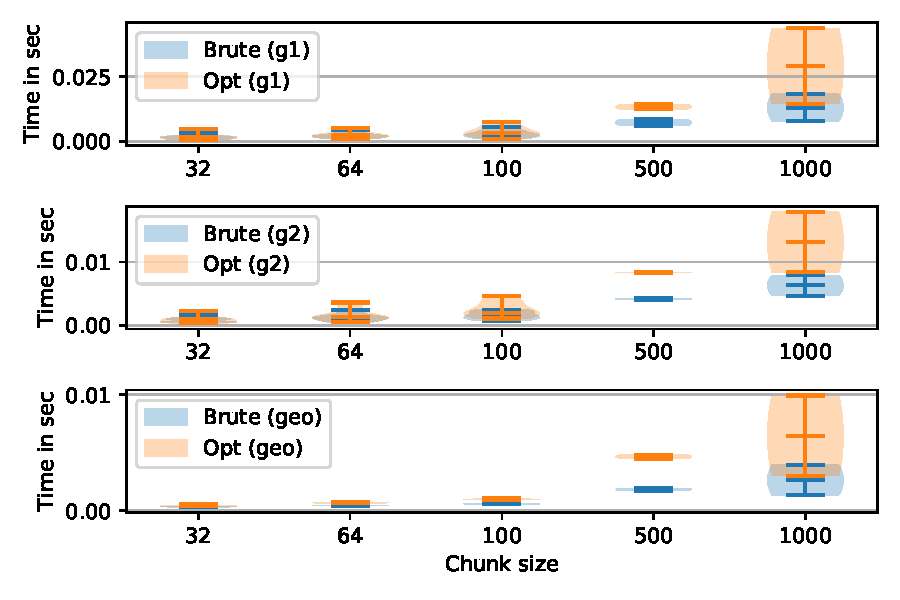
\includegraphics[width=\textwidth]{data/raw/core.pdf}
         \caption{$y=x$}
         \label{fig:y equals x}
     \end{subfigure}
     ~\begin{subfigure}[b]{0.24\textwidth}
         \centering
         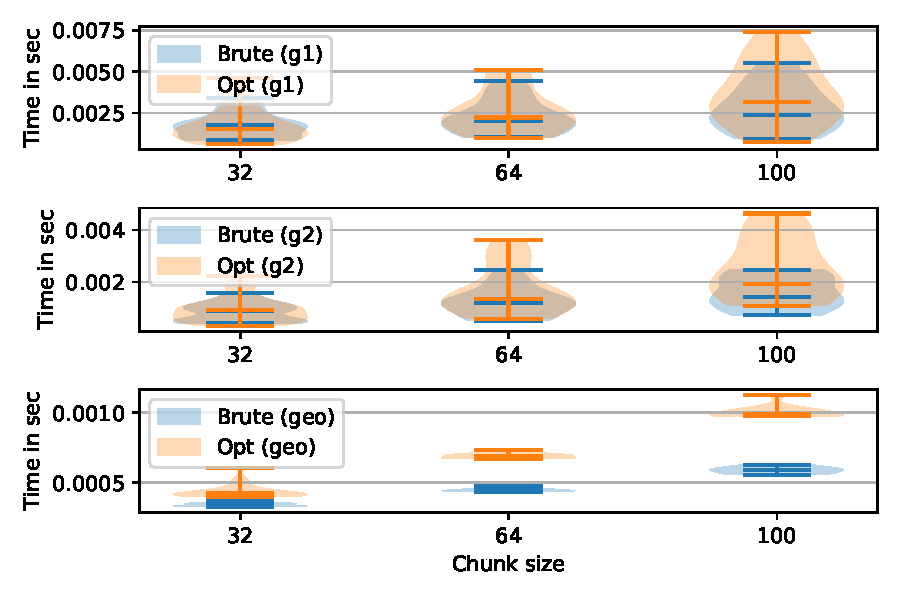
\includegraphics[width=\textwidth]{data/raw/core_3.pdf}
         \caption{$y=x$}
         \label{fig:y equals x}
     \end{subfigure}\\
   \caption{Single path extraction}
\end{figure}


\begin{figure}[h]
\centering
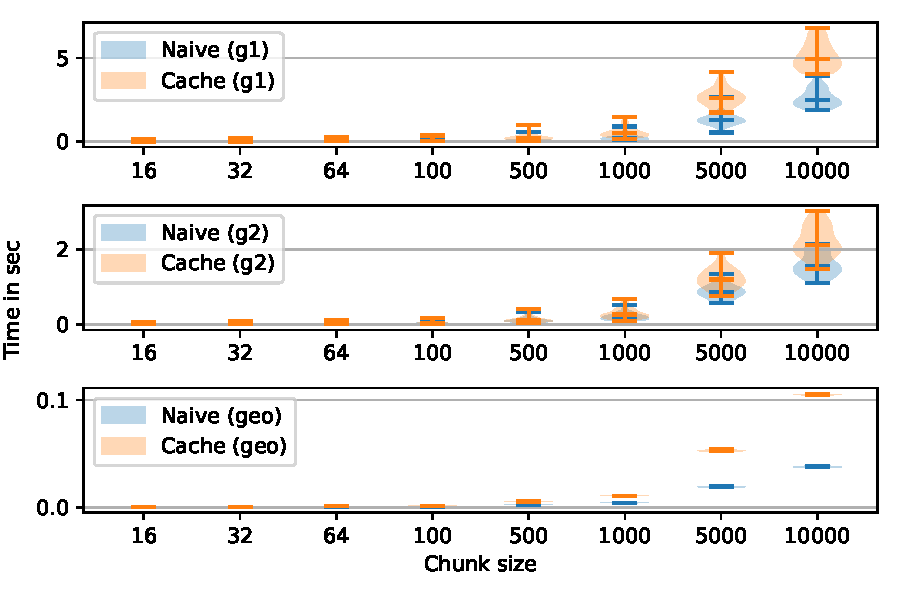
\includegraphics[width=0.5\textwidth]{data/raw/go.pdf}
\caption{Example of a parametric plot ($\sin (x), \cos(x), x$)}
\end{figure}

\begin{figure}[h]
\centering
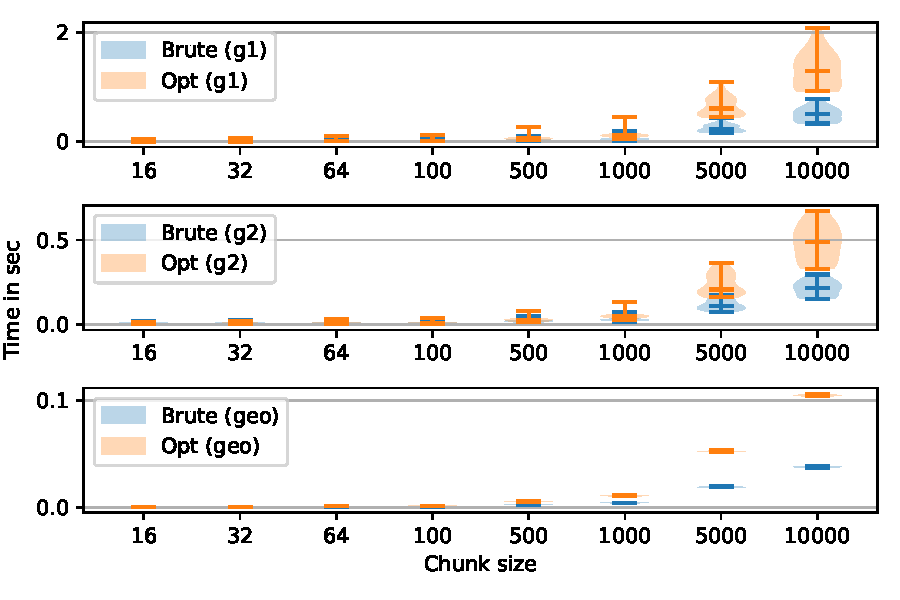
\includegraphics[width=0.5\textwidth]{data/raw/eclass_514en.pdf}
\caption{Example of a parametric plot ($\sin (x), \cos(x), x$)}
\end{figure}

\begin{figure}[h]
\centering
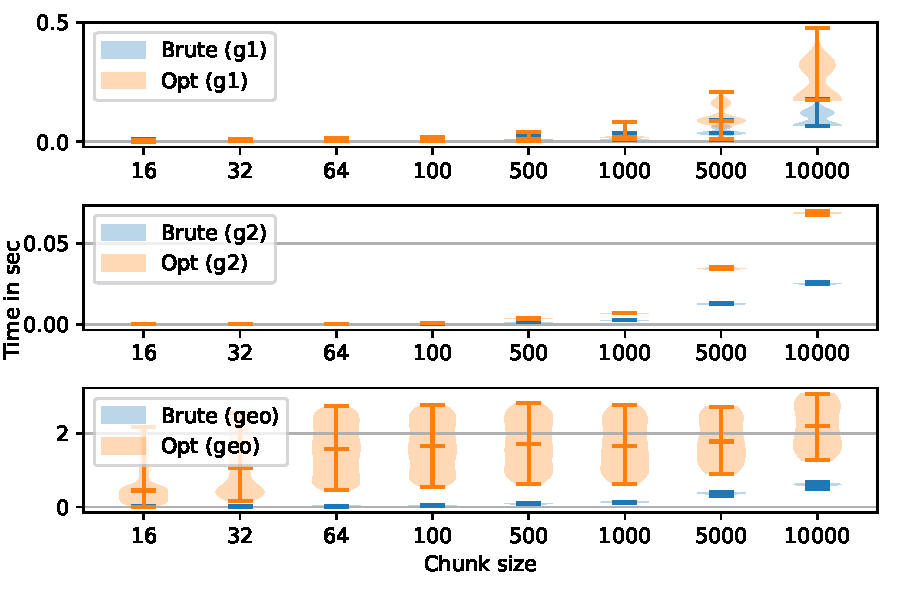
\includegraphics[width=0.5\textwidth]{data/raw/geospecies.pdf}
\caption{Example of a parametric plot ($\sin (x), \cos(x), x$)}
\end{figure}

\begin{figure}[h]
\centering
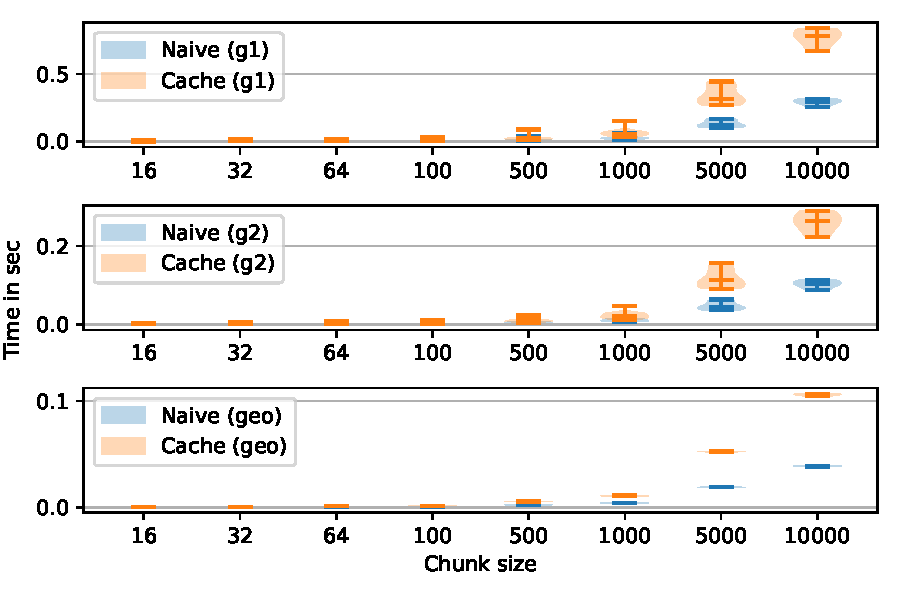
\includegraphics[width=0.5\textwidth]{data/raw/enzyme.pdf}
\caption{Example of a parametric plot ($\sin (x), \cos(x), x$)}
\end{figure}

\begin{figure}[h]
\centering
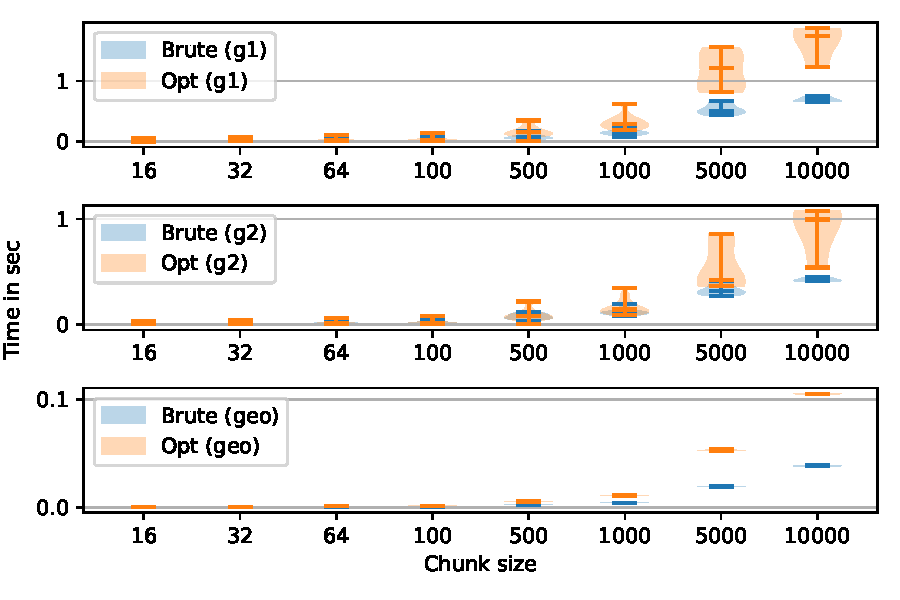
\includegraphics[width=0.5\textwidth]{data/raw/gohierarchy.pdf}
\caption{Example of a parametric plot ($\sin (x), \cos(x), x$)}
\end{figure}


\begin{figure}[h]
\centering
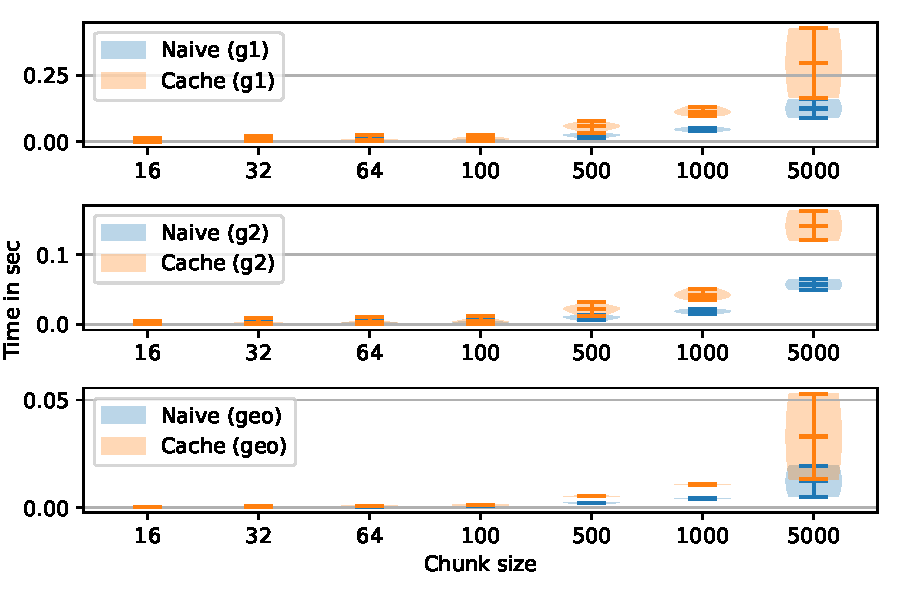
\includegraphics[width=0.5\textwidth]{data/raw/pathways.pdf}
\caption{Example of a parametric plot ($\sin (x), \cos(x), x$)}
\end{figure}


Results.

Conclusion. 
\section{CFPQ Full-Stack Support}

In order to provide full-stack support of CFPQ it is necessatry to choose an appropriate graph database.
It was shown by Arseniy Terekhov et al. in~\cite{10.1145/3398682.3399163} that matrix-based algorithm can be naturally integrated into RedisGraph graph database because both, the algorithm and the database, operates over matrix representation of graphs.
Moreover, RedisGraph supports Cypher as a query language and there is a proposal which describes Cypher extension which allows one to specify context-free constraints.
Thus we choose RedisGraph as a base for our solution.  


\subsection{Cypher Extending}
\label{subsec:cypher-extension}

The first what we should do is to extend Cypher parser to be able to express context-free constraints.
There is a description of the respective Cypher syntax extension\footnote{\label{cypher-proposal}Formal syntax specification: \url{https://github.com/thobe/openCypher/blob/rpq/cip/1.accepted/CIP2017-02-06-Path-Patterns.adoc\#11-syntax}. Access date: 19.07.2020.}, proposed by Tobias Lindaaker, but this syntax does not implement yet in Cypher parsers.

This extension introduces path patterns, which are powerful alternative to the original Cypher relationship patterns.
Path patterns allow one to express regular constrains over basic patterns such as relationship and node patterns.
Like relationship patterns, they can be specified in the \texttt{MATCH} clause.

Main feature which allows one to specify context-free constraints is a \textit{named path patterns}: one can specify a name for path pattern and after that use this name in other patterns, or in the same pattern.
Named patterns can be defined in the \texttt{PATH PATTERN} clause.
Using this feature, structure of query is pretty similar to context-free grammar in the Extended Backus-Naur Form (EBNF)~\cite{EBNF_ISO}.

\begin{algorithm}
\floatname{algorithm}{Listing}
\begin{algorithmic}[1]
\caption{Query based on example grammar $G_1$ (eq.~\ref{eqn:g1_example}) in Cypher with path patterns}
\label{lst:cypher_example}
\State PATH PATTERN S = ()-/ [:c $\sim$S :d] | [:c (:y) :d] /->()
\State MATCH (v:x)-[:a | :c]->()-/ :b $\sim$S /->(to)
\State RETURN v, to
\end{algorithmic}
\end{algorithm}


The example of query which uses named path patters is presented in listing~\ref{lst:cypher_example}. 
This query is based on context-free grammar $G_1$ (eq.~\ref{eqn:g1_example}). 
Namely, path patter with name \texttt{S} specifies exactly the same constraint that specified by the grammar $G_1$. 
The \texttt{MATCH} clause uses pattern \texttt{S} in complex constraint which says that path of interest should starts in the vertex with label \texttt{x}, than in should goes throw edge with label \texttt{a} or \texttt{c}, and the end of path is a sequence of edges which starts from \texttt{b} and tail of this sequence matches with \texttt{S}.  

For the example graph $D_1$ this query returns the next pairs of vertices \texttt{(v, to)} (as specified in \texttt{RETURN} clause): !!!!

Thus this Cypher extension allows one express more complex queries including context-free path queries.
RedisGraph database supports subset of Cypher language and uses \texttt{libcypher-parser}\footnote{The \texttt{libcypher-parser} is an open-source parser library for Cypher query language. GitHub repository of the project: \url{https://github.com/cleishm/libcypher-parser}. Access date: 19.07.2020.} library to parse queries.
We extend this library by introducing new syntax proposed.
Note that we implement\footnote{The modified libsypher-pareser library with support of syntax for path patterns: \url{https://github.com/YaccConstructor/libcypher-parser}. Access date: 19.07.2020.} full extension, not only part which is necessary for simple CFPQ. 

\subsection{RedisGraph Extending}

This section describes the implementation of support for executing queries with the extended syntax in the RedisGraph. Throughout this section, we consider executing the example query from listing~\autoref{lst:cypher-example-3} for the graph $D_1$ from~\autoref{fig:example_input_graph}. $\mathcal{E}$ and $\mathcal{V}$ denotes boolean decompositions of adjacency and vertex label matrices of $D_1$ respectively. 

In the RedisGraph the main part of processing a query is building its execution plan. Execution plan consists of operations that perform basic processing such as filtering, pattern matching, aggregation and result construction. The diagram of its construction is shown in~\autoref{fig:execution-plan-construction}

After obtaining algebraic expressions they are used to construct execution plan operations. Each operation is derived from a single algebraic expression that is involved in the further execution of the corresponding operation.  During the query execution this operation performs path pattern matching and solves context-free path reachability problem if necessary. This completes the part of the query execution plan building which concerns unnamed path patterns.


The remaining part of query processing is evaluation its execution plan.

Let`s first consider the structure of the execution plan operations. Operations have parent-child relationships, so they are formed into a tree. For example, the part of execution plan that derived from example query is shown in~\autoref{fig:execution-plan-operations}. Each operation can consume a record from a child operation, process it and produce another one for the parent. Records contain information necessary for the parent operation, as well as everything to restore the response, such as identifiers of accumulated vertices and edges.


\subsection{Evaluation}

In order to demonstrate applicability of the provided extension for RedisGraph we evaluate the proposed solution on the subset of cases provided in the section~\ref{sect:py_algo_evaluation}.

For RedisGraph evaluation, we used a PC with Ubuntu 18.04 installed.
It has Intel Core i7-6700 CPU, 3.4GHz, and DDR4 64Gb RAM. 
RedisGraph with our extensions is installed form our GitHub repository\footnote{Sources of RedisGraph database with full-stack CFPQ support:\url{https://github.com/YaccConstructor/RedisGraph/tree/path_patterns_dev}. Access data: 19.07.2020.}. 

\subsubsection{Data preparing}

We use the same graphs which are presented in table~\ref{tbl:graphs_for_cfpq} to evaluate RedisGraph-based solution.

Graphs are loaded into RedisGraph database such that each vertex has a field \verb|id| which value is unique and is in $[0 \ldots |V|-1]$, where $|V|$ is a number of vertices in the graph to load.
This allows us to generate queries for specific chunk size using templates.
The template for the $g_1$ query is provided in listing~\ref{lst:query_pattern_g1}.
Here \texttt{\{id\_from\}} and \texttt{\{id\_to\}} are placeholders for lower and upper bounds for \verb|id|. The example of the exact query for chunk of size 16 is presented in listing~\ref{lst:query_g1}.

\begin{algorithm}
\floatname{algorithm}{Listing}
\begin{algorithmic}[1]
\caption{Cypher query pattern for $g_1$}
\label{lst:query_pattern_g1}
\State PATH PATTERN S =  \par
 \hskip\algorithmicindent ()-/ [<:SubClassOf [$\sim$S | ()] :SubClassOf] \par
 \hskip\algorithmicindent | [<:Type [$\sim$S | ()] :Type] /->()
\State MATCH (src)-/ $\sim$S /->() 
\State WHERE \{id\_from\} <= src.id and src.id <= \{id\_to\}
\State RETURN count(*)
\end{algorithmic}
\end{algorithm}

\begin{algorithm}
\floatname{algorithm}{Listing}
\begin{algorithmic}[1]
\caption{Query $g_1$ in Cypher using the template from listing~\ref{lst:query_pattern_g1}}
\label{lst:query_g1}
\State PATH PATTERN S =  \par
 \hskip\algorithmicindent ()-/ [<:SubClassOf [$\sim$S | ()] :SubClassOf] \par
 \hskip\algorithmicindent | [<:Type [$\sim$S | ()] :Type] /->()
\State MATCH (src)-/ $\sim$S /->() 
\State WHERE 15 <= src.id and src.id <= 31
\State RETURN count(*)
\end{algorithmic}
\end{algorithm}

Queries generator for all three queries ($g_1$, $g_2$, and $geo$) was implemented and used to create queries for all chunks which are used in the previous experiment. 


\subsubsection{Evaluation results}

For evaluation we select $geo$ query for \textit{geospecies} graph as one of the hardest queries, and $g_1$ query for other graphs.
Time and memory consumption are measured for each chunk processing.
Results of time measurement are presented in figures~\ref{fig:redis_core_all}--\ref{fig:redis_gohierarchy_all}.

\begin{figure}[h]
\centering
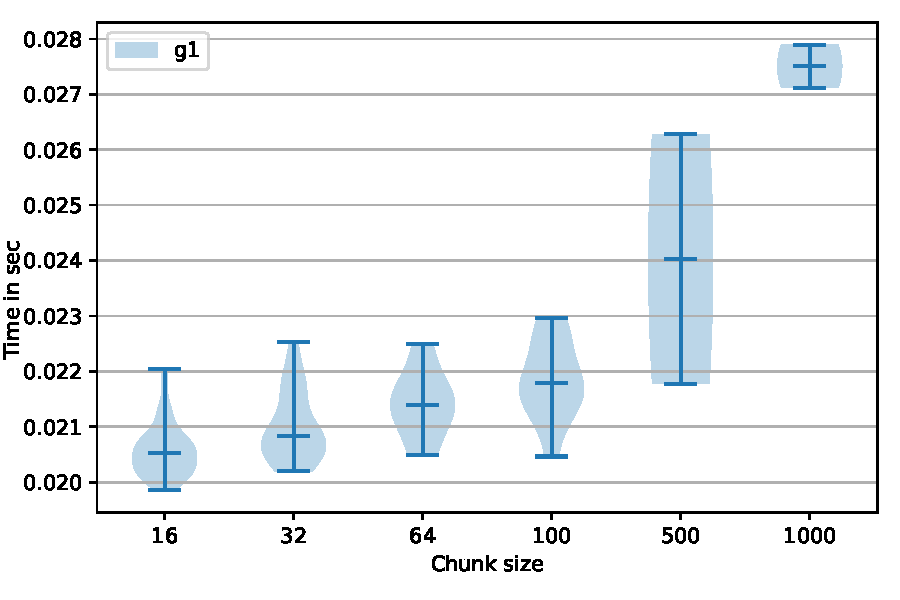
\includegraphics[width=0.45\textwidth]{data/raw_redis/core.pdf}
\caption{RedisGraph performance on \textit{core} graph}
\label{fig:redis_core_all}
\end{figure}


\begin{figure}[h]
\centering
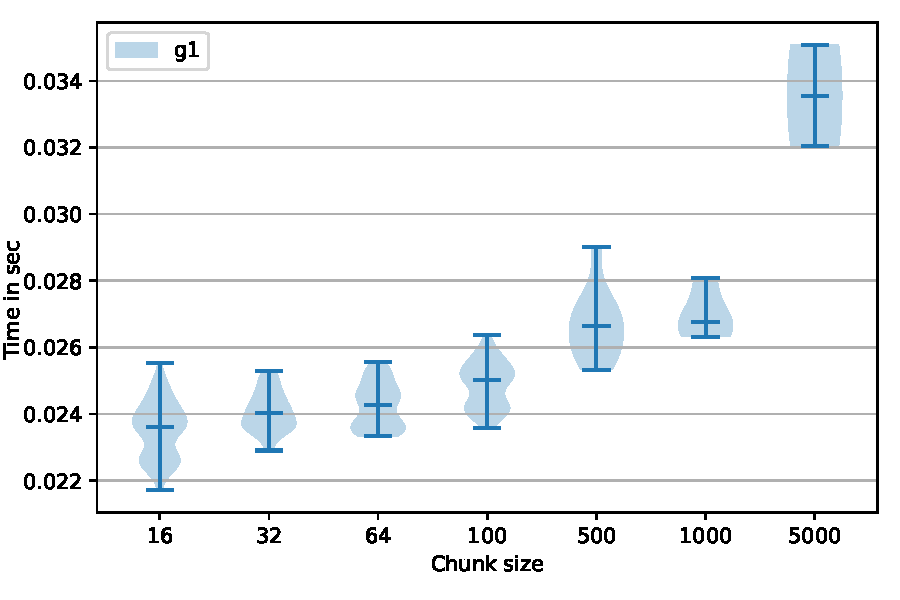
\includegraphics[width=0.45\textwidth]{data/raw_redis/pathways.pdf}
\caption{RedisGraph performance on \textit{pathways} graph}
\label{fig:redis_pathways_all}
\end{figure}

\begin{figure}[h]core
\centering
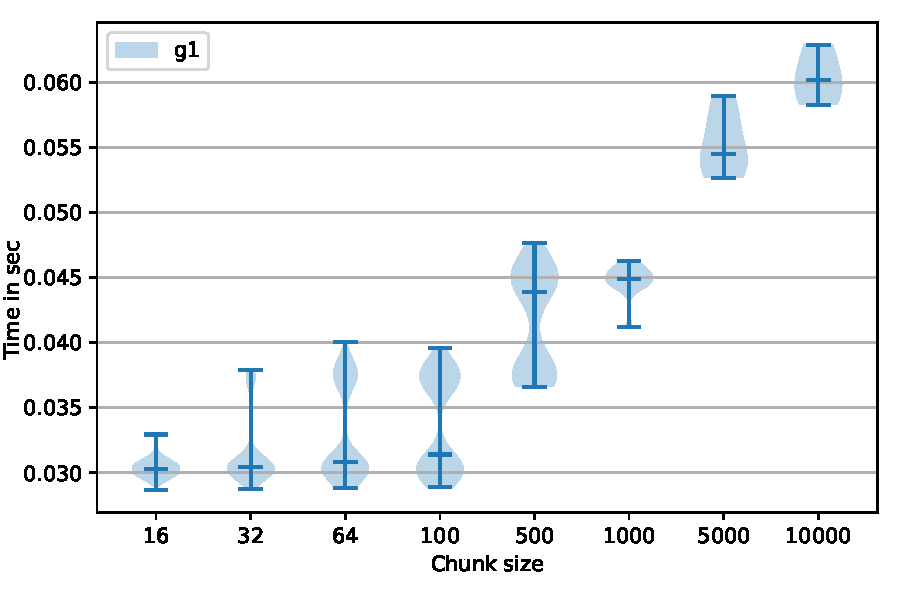
\includegraphics[width=0.45\textwidth]{data/raw_redis/enzyme.pdf}
\caption{RedisGraph performance on \textit{enzyme} graph}
\label{fig:redis_enzyme_all}
\end{figure}


\begin{figure}[h]
\centering
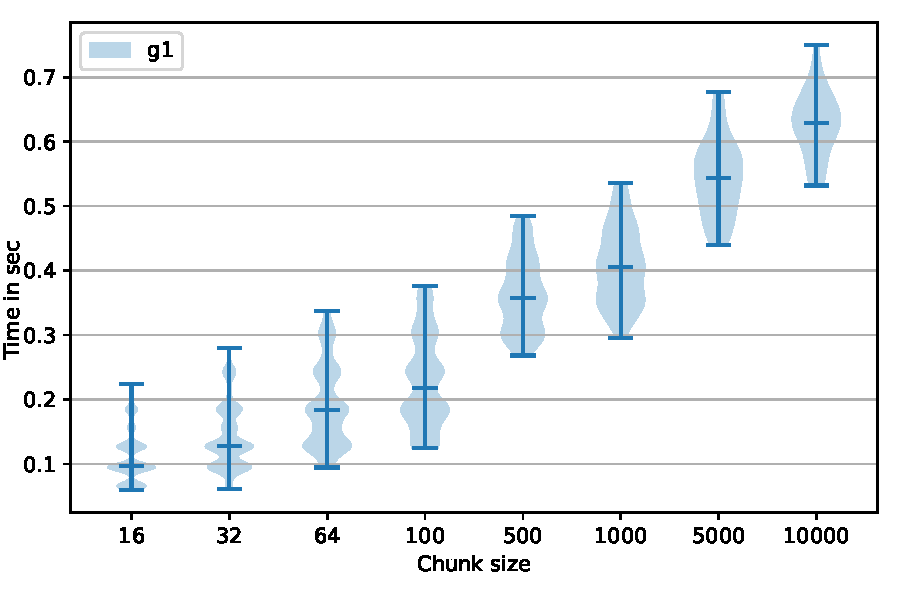
\includegraphics[width=0.45\textwidth]{data/raw_redis/go.pdf}
\caption{RedisGraph performance on \textit{go} graph}
\label{fig:redis_go_all}
\end{figure}

\begin{figure}[h]
\centering
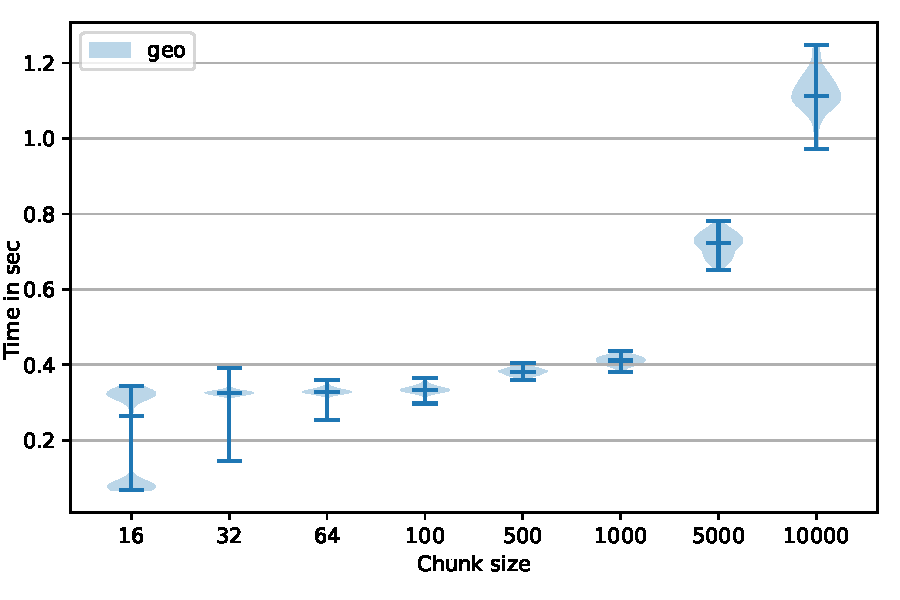
\includegraphics[width=0.45\textwidth]{data/raw_redis/geospecies.pdf}
\caption{RedisGraph performance on \textit{geospecies} graph}
\label{fig:redis_geospecies_all}
\end{figure}

\begin{figure}[h]
\centering
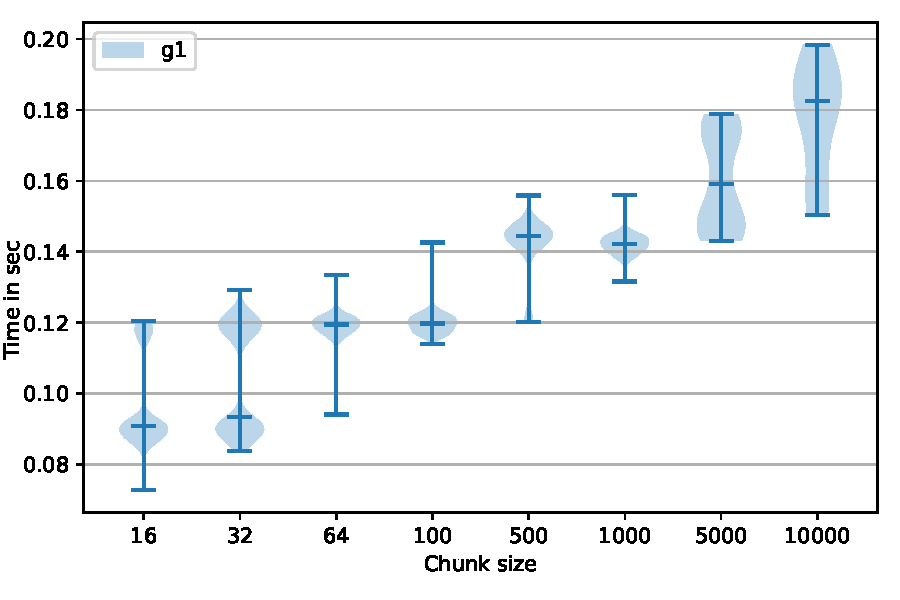
\includegraphics[width=0.45\textwidth]{data/raw_redis/eclass_514en.pdf}
\caption{RedisGraph performance on \textit{eclass\_514en} graph}
\label{fig:redis_eclass_all}
\end{figure}

\begin{figure}[h]
\centering
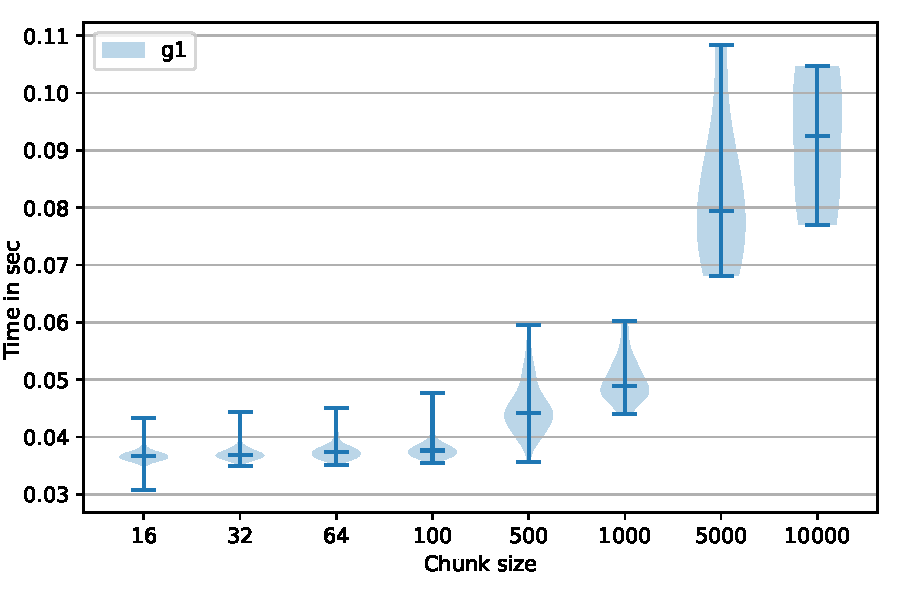
\includegraphics[width=0.45\textwidth]{data/raw_redis/gohierarchy.pdf}
\caption{RedisGraph performance on \textit{gohierarchy} graph}
\label{fig:redis_gohierarchy_all}
\end{figure}

We can see, that results is comparable with one given in section~\ref{sect:py_algo_evaluation}. 
Processing time for all chunks, except chunk of size 10~000 for \textit{geospecies} graph (fig.~\ref{fig:redis_geospecies_all}) is less then 1 second.
Moreover, for chunks of size 16 processing median time is less then 0.1 second, except \textit{geospecies} graph.

Memory consumption for two big graphs \textit{eclass\_514en} and \textit{geospecies} is presented in figures~\ref{fig:redis_memory_eclass} and~\ref{fig:redis_memory_geospecies} respectively.
We can see, that amount of used memory depends on graph and query, but for relatively small chunks ($\leq 1000$) RedisGraph uses less that 50Mb of RAM to process one chunk.
Note that RedisGraph includes memory management system, thus in our experiments all allocated memory is measured, not only really used for query evaluation.
As a result, we can conclude that multiple-source CFPQ is significantly more memory efficient than creation of full reachability index and its filtering: processing the chunk of size 10~000 on \textit{geospecies} graph requires less than 200Mb, while full index creation requires 16Gb~\cite{10.1145/3398682.3399163}.  

\begin{figure}[h]
\centering
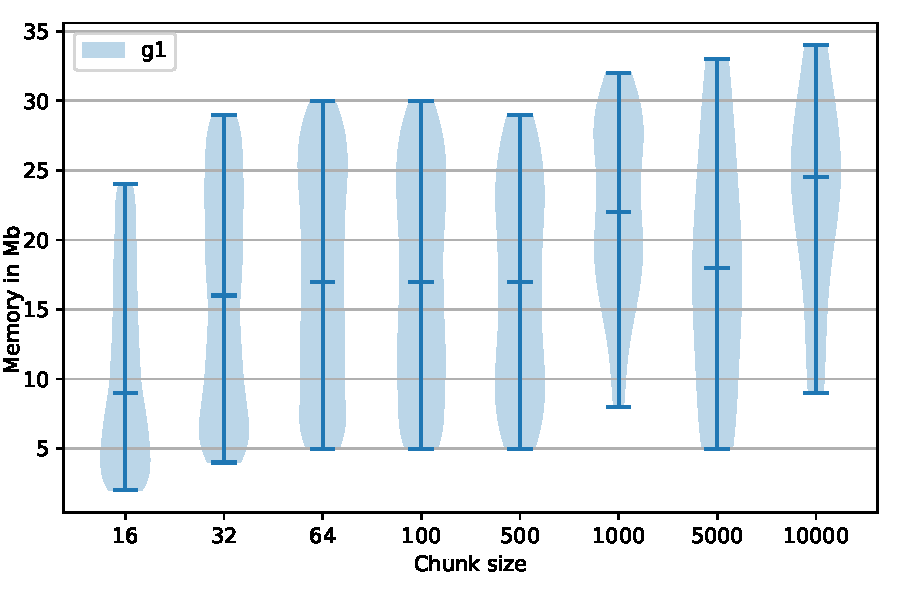
\includegraphics[width=0.5\textwidth]{data/raw_memory/eclass_514en.pdf}
\caption{RedisGraph memory consumption on \textit{eclass\_514en} graph}
\label{fig:redis_memory_eclass}
\end{figure}

\begin{figure}[h]
\centering
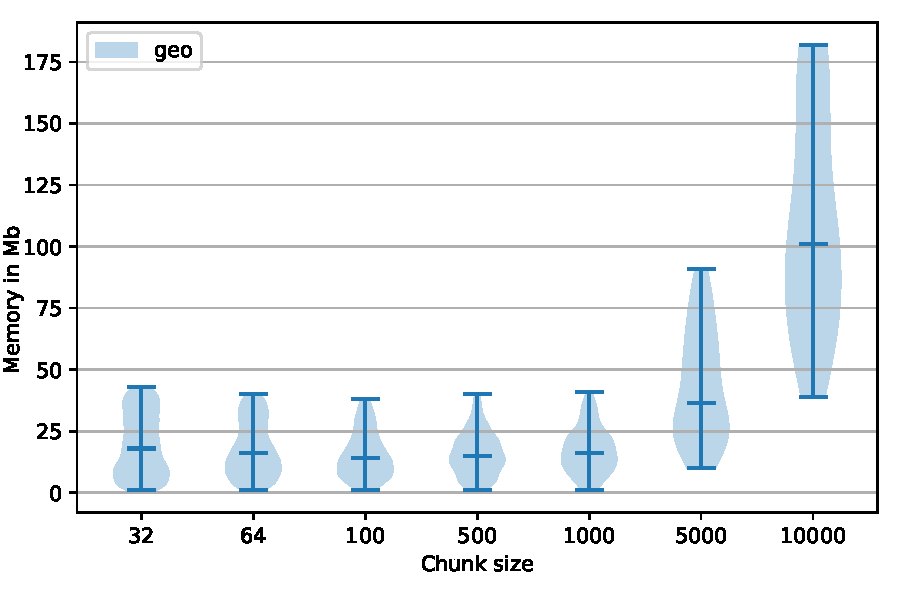
\includegraphics[width=0.5\textwidth]{data/raw_memory/geospecies.pdf}
\caption{RedisGraph memory consumption on \textit{geospecies} graph}
\label{fig:redis_memory_geospecies}
\end{figure}


\begin{algorithm}
\floatname{algorithm}{Listing}
\begin{algorithmic}[1]
\caption{Query $g_1$ in Cypher for all-pairs scenario evaluation}
\label{lst:query_g1_full}
\State PATH PATTERN S =  \par
 \hskip\algorithmicindent ()-/ [<:SubClassOf [$\sim$S | ()] :SubClassOf] \par
 \hskip\algorithmicindent | [<:Type [$\sim$S | ()] :Type] /->()
\State MATCH ()-/ $\sim$S /->() 
\State RETURN count(*)
\end{algorithmic}
\end{algorithm}


Additionally, we measure the time required to process full graph (to solve all-pairs reachability problem) by chunks of size 1000.
Namely, we evaluate the qury, presented in listing~\ref{lst:query_g1_full}. 
It is similar to query form the previous scenario, but without constraints on vertices ids (without \texttt{WHERE} clause).
Total processing time (in seconds) and total required memory (in Mb) are measured.
Also, we compare our solution with results of Arseniy Terekhov et al. from~\cite{10.1145/3398682.3399163} which were measured for RedisGraph deployed on the similar hardware and for the same graphs and queries.
In~\cite{10.1145/3398682.3399163} Azimov's algorithm was naively integrated with RedisGraph storage without support of query language and other mechanisms such as lazy query evaluation.
Results are provide in the table~\ref{tbl:redis_full_graph_processing}.

{\setlength{\tabcolsep}{0.25em}
\begin{table}
{
\caption{Full graph processing time by RadisGraph with chunks of size 1000, time is measured in seconds, memory in Mb (\textbf{Chunks} --- the proposed solution, \textbf{Mono} --- results from~\cite{10.1145/3398682.3399163})}
\label{tbl:redis_full_graph_processing}
\small
\rowcolors{3}{black!2}{black!10}
\begin{tabular}{|l|c|c|c|c|c|c|}
\hline
\multirow{2}{*}{Graph} & \multirow{2}{*}{\#V} & \multirow{2}{*}{\#E} & \multirow{2}{*}{Query} & \multicolumn{2}{c|}{Chunks}  &  \multirow{2}{*}{Mono}  \\
                       &                      &                      &                        & Time   & Mem & \\
\hline
\hline
core                   & 1323                 & 3636                 & $g_1$                  & 0.003  & 2                  &  0.004 \\ 
pathways               & 6238                 & 18 598               & $g_1$                  & 0.031  & 6                  &  0.011 \\ 
gohierarchy            & 45 007               & 980 218              & $g_1$                  & 0.847  & 62                  &  0.091 \\ 
enzyme                 & 48 815               & 117 851              & $g_1$                  & 0.698  & 13                  &  0.018 \\ 
eclass\_514en          & 239 111              & 523 727              & $g_1$                  & 18.825 & 35                   &  0.067 \\ 
geospecies             & 450 609              & 2 311 461            & $geo$                  & 80.979 & 196                  &  7.146 \\
go                     & 582 929              & 1 758 432            & $g_1$                  & 72.034 & 40                  &  0.604 \\ 
\hline
\end{tabular}
}
\end{table}
}

We can see, that chunk-by-chunk processing is slower, but it is still require reasonable time.
First of all, if chunk size is comparable with graph size (\textit{core} and \textit{pathways} graphs) then time to processing is comparable with monolithic processing.
Thus one can decrease time to process by increasing of chunk size and gets near optimal time.
On the other hand, even with relatively small chunks (\textit{eclass\_514}, \textit{go} and \textit{geospecies} graphs), when for chunk-by-chunk processing requires more than 100 times more time, our results still reasonable for some cases. 
For example, it requires more than 70 times less time for \textit{geospecies} grap processing than solution of Jochem Kuijpers et al.~\cite{Kuijpers:2019:ESC:3335783.3335791} which is based on Neo4j and requires more than 6000 seconds.
Moreover, while solution from~\cite{10.1145/3398682.3399163} requires huge amount of memory (more than 16Gb for \textit{geospecies} graph and $geo$ query), our solution requires only 196Mb in the same scenario.
Thus it is more suitable for general-purpose graph databases: main scenario---relatively small start vertices set---can be handled efficiently, and all-pairs reachability, which is not a massive case, can be solved in reasonable time with low memory consumption. In specific cases one can easy tune our solution to get optimal time and memory consumption.

Finally we can conclude that provided solution is a promising way to implement CPFQ for real-world graph databases.
%\section{Evaluation}

We evaluate the implemented algorithm on both regular and context-free path queries in order to demonstrate applicability of the proposed solution.
Namely, goals of the evaluation are following.
\begin{enumerate}
	\item Investigate the practical applicability of RPQ evaluation by the proposed algorithm.
	\item Compare Azimov's algorithm for reachability CFPQ and the proposed algorithm.
	\item Investigate the practical applicability of paths extraction algorithm for both regular and context-free queries.
\end{enumerate}

For evaluation, we use a PC with Ubuntu 18.04 installed.
It has Intel core i7-6700 CPU, 3.4GHz, and DDR4 64Gb RAM.
As far as we evaluate only algorithm execution time, we store each graph fully in RAM as its adjacency matrix in sparse format.
Note, that graph loading time is not included in the result time of evaluation.	

\subsection{RPQ Evaluation}

In oder to investigate applicability of the proposed algorithm for RPQ over real-world graphs we collect a set of real-world and synthetic graphs and evaluate queries generated by using the most popular templates for RPQs.

\subsubsection{Dataset}

Brief description of collected graphs are presented in Table~\ref{tbl:graphs_for_rpq}.
Namely, the dataset consists of several parts.
The first one is a set of LUBM graphs\footnote{Lehigh University Benchmark (LUBM) web page: \url{http://swat.cse.lehigh.edu/projects/lubm/}. Access date: 07.07.2020.}~\cite{10.1016/j.websem.2005.06.005} with a different number of vertices.
The second one is a graphs from Uniprot database\footnote{Universal Protein Resource (UniProt) web page: \url{https://www.uniprot.org/}. All files used for evaluation can be downloaded here: \url{ftp://ftp.uniprot.org/pub/databases/uniprot/current_release/rdf/}. Access date: 07.07.2020.}: \textit{proteomes}, \textit{taxonomy} and \textit{uniprotkb}.
The last part is a RDF files \textit{mappingbased\_properties} from DBpedia\footnote{DBpedia project web site: \url{https://wiki.dbpedia.org/}. Access date: 07.07.2020.} and \textit{geospecies}\footnote{The Geospecies RDF: \url{https://old.datahub.io/dataset/geospecies}. Access date: 07.07.2020.}.
These graphs represent data from different areas and they are frequently used for graph querying algorithms evaluation.

\begin{table}
{
\rowcolors{2}{black!2}{black!10}
\begin{tabular}{|l|c|c|}
\hline
Graph & \#V & \#E \\
\hline
\hline 
LUBM1k  & 120 926 & 484 646 \\
LUBM3.5k  & 358 434 & 144 9711 \\
LUBM5.9k  & 596 760 & 2 416 513 \\
LUBM1M   & 1 188 340 & 4 820 728 \\
LUBM1.7M & 1 780 956 & 7 228 358 \\
LUBM2.3M & 2 308 385 & 9 369 511 \\
\hline
Uniprotkb & 6 442 630 & 24 465 430 \\
Proteomes & 4 834 262 & 12 366 973 \\
Taxonomy & 5 728 398 & 14 922 125 \\
\hline
Geospecies & 450 609 & 2 201 532 \\
Mappingbased\_properties & 8 332 233 & 25 346 359 \\
\hline
\end{tabular}
}
\caption{Graphs for RPQ evaluation}
\label{tbl:graphs_for_rpq}
\end{table}


Queries for evaluation was generated by using templates of the most popular RPQs which are collected from~
\cite{Pacaci2020RegularPQ} (Table 2) and~\cite{Wang2019} (some of complex queries from Table 5), and are presented in table~\ref{tbl:queries_templates}.
We generate 10 queries for each template and each graph using the most frequent relations from the given graph randomly\footnote{Used generator is available as part of CFPQ\_data project: \url{https://github.com/JetBrains-Research/CFPQ_Data/blob/master/tools/gen_RPQ/gen.py}. Access data: 07.07.2020.}. 
For all LUBM graphs common set of queries was generated in order to investigate scalability of the proposed algorithm.

\begin{table}
{\small
\renewcommand{\arraystretch}{1.25}
\rowcolors{2}{black!2}{black!10}
\begin{tabular}{|c|c||c|c|}
\hline

Name & Query & Name & Query \\
\hline
\hline 
$Q_1$   & $a^*$                               & $Q_9^5$    & $(a \mid b \mid c \mid d \mid e)^+$                     \\
$Q_2$   & $a\cdot b^*$                        & $Q_{10}^2$ & $(a \mid b) \cdot c^*$                                  \\
$Q_3$   & $a \cdot b^* \cdot c^*$             & $Q_{10}^3$ & $(a \mid b \mid c)  \cdot d^*$                          \\
$Q_4^2$ & $(a \mid b)^*$                      & $Q_{10}^4$ & $(a \mid b \mid c \mid d)  \cdot e^*$                   \\
$Q_4^3$ & $(a \mid b \mid c)^*$               & $Q_{10}^5$ & $(a \mid b \mid c \mid d \mid e)  \cdot f^*$            \\
$Q_4^4$ & $(a \mid b \mid c \mid d)^*$        & $Q_{10}^2$ & $a \cdot b$                                             \\
$Q_4^5$ & $(a \mid b \mid c \mid d \mid e)^*$ & $Q_{11}^3$ & $a \cdot b \cdot c$                                     \\
$Q_5$   & $a \cdot b^* \cdot c$               & $Q_{11}^4$ & $a \cdot b \cdot c \cdot d$                             \\
$Q_6$   & $a^* \cdot b^*$                     & $Q_{11}^5$ & $a \cdot b \cdot c \cdot d \cdot f$                     \\
$Q_7$   & $a \cdot b \cdot c^*$               & $Q_{12}$   & $(a \cdot b)^+ \mid  (c \cdot d)^+$                     \\
$Q_8$   & $a? \cdot b^*$                      & $Q_{13}$   & $(a \cdot(b \cdot c)^*)^+ \mid  (d \cdot f)^+$          \\
$Q_9^2$ & $(a \mid b)^+$                      & $Q_{14}$   & $(a \cdot b \cdot (c \cdot d)^*)^+  \cdot (e \mid f)^*$ \\
$Q_9^3$ & $(a \mid b \mid c)^+$               & $Q_{15}$   & $(a \mid b)^+ \cdot (c \mid d)^+$                       \\
$Q_9^4$ & $(a \mid b \mid c \mid d)^+$        & $Q_{16}$   & $a \cdot b \cdot (c \mid d \mid e)$                     \\
\hline
\end{tabular}
}
\caption{Queries' templates for RPQ evaluation}
\label{tbl:queries_templates}
\end{table}


\subsubsection{Results}

For reachability index creation average time of 5 runs is presented.

Reachability index creation time for each query for LUBM graphs set is presented in figure~\ref{fig:lubm_all_qs}.
We can observe linear !!!! dependency of evaluation time on graph size.
Also we can see, that query evaluation time depends on query: there are queries which evaluate less then 1 second even for biggest graph ($Q_2$, $Q_5$, $Q_{11}^2$, $Q_{11}^3$), while worst time is 6.26 seconds ($Q_{14}$).
Anyway, we can argue that in this case our algorithm demonstrates reasonable time to be applied for real-world data analysis, because it is comparable with recent results on the same problem for LUBM querying by using distributed system over 10 nodes~\cite{Wang2019}, while we use only one node. 
Note, that accurate comparison of different approaches is a huge interesting work for the future.

\begin{figure}
   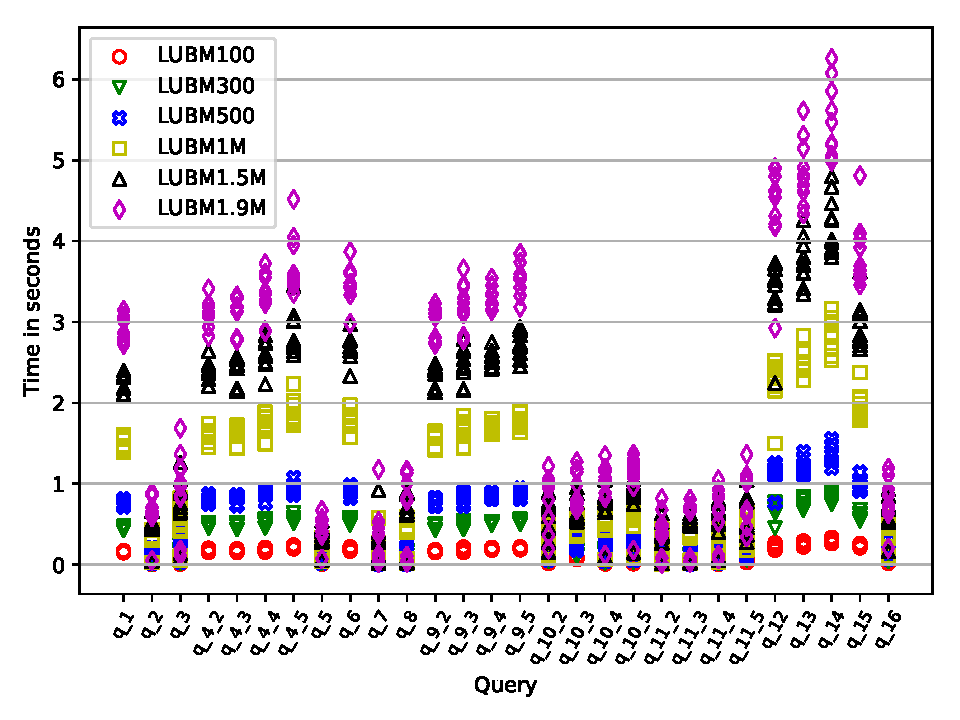
\includegraphics[width=0.48\textwidth]{data/LUBM_all.pdf}
   \caption{Reachability index creation time for LUBM graphs}
   \label{fig:lubm_all_qs}
\end{figure}

Reachability index creation time for each query for for real-world graphs is presented in figure~\ref{fig:other_all_qs}.
We can see that query evaluation time depends on graph inner structure. 
First of all, in some cases handling of small graph requires more time, then handling bigger graph.
For example, $Q_{10}^4$: querying the \textit{geospecies} graph (450k vertices) in some cases requires more time than querying of \textit{mappingbased\_properties} (8.3M vertices) and \textit{taxonomy} (5.7M vertices).
On the other hand, \textit{taxonomy} querying in relatively big number of cases requires significantly more time, than querying of other graphs, while \textit{taxonomy} is not a biggest graph. 
Finally, we can see, that in big number of cases query execution time requires less then 10 seconds, even for big graph, and no queries which require more then 52.17 seconds. 

\begin{figure}
   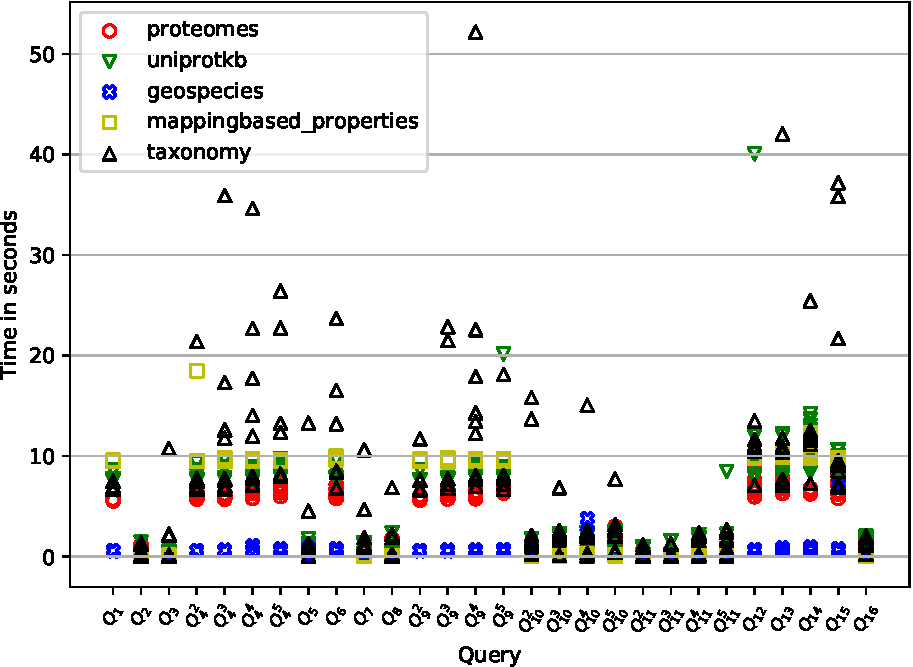
\includegraphics[width=0.48\textwidth]{data/other_all.pdf}
   \caption{Reachability index creation time for real-world RDFs}
   \label{fig:other_all_qs}
\end{figure}

Paths extraction was evaluated on cases with possible long paths.
These cases were selected during reachability index creation by using number of iterations in transitive closure evaluation.
For each selected graph and query we measure paths extraction time for each reachable pair, reachability index creation time is not included because exactly the same index, as calculated at the previous step, is used for paths extraction. 

We evaluate two scenarios.
The first one is a single path extraction.
In this case results are represented as a dependency of extraction time on extracted path length.
We can see linear !!!!

The second scenario is many paths extraction.
Here we limit a number of path to extract by !!! 
In this case results are represented as a dependency of extraction time on number of extracted paths.


\begin{figure}
     \begin{subfigure}[b]{0.24\textwidth}
         \centering
         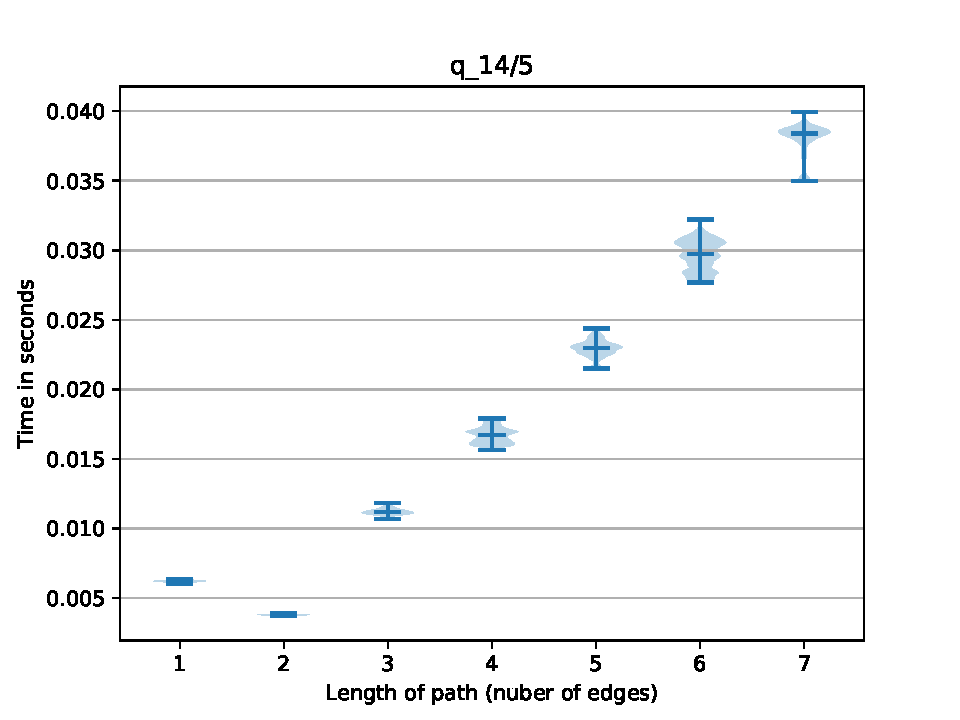
\includegraphics[width=\textwidth]{data/res_graphics/q_14_5.pdf}
         \caption{$y=x$}
         \label{fig:y equals x}
     \end{subfigure}
     ~\begin{subfigure}[b]{0.24\textwidth}
         \centering
         %\includegraphics[width=\textwidth]{data/res_graphics/q9_2_8.pdf}
         \caption{$y=x$}
         \label{fig:y equals x}
     \end{subfigure}\\
     \begin{subfigure}[b]{0.24\textwidth}
         \centering
         %\includegraphics[width=\textwidth]{data/res_graphics/q_14_8.pdf}
         \caption{$y=x$}
         \label{fig:y equals x}
     \end{subfigure}
     ~\begin{subfigure}[b]{0.24\textwidth}
         \centering
         %\includegraphics[width=\textwidth]{data/res_graphics/q4_2_8.pdf}
         \caption{$y=x$}
         \label{fig:y equals x}
     \end{subfigure}
   %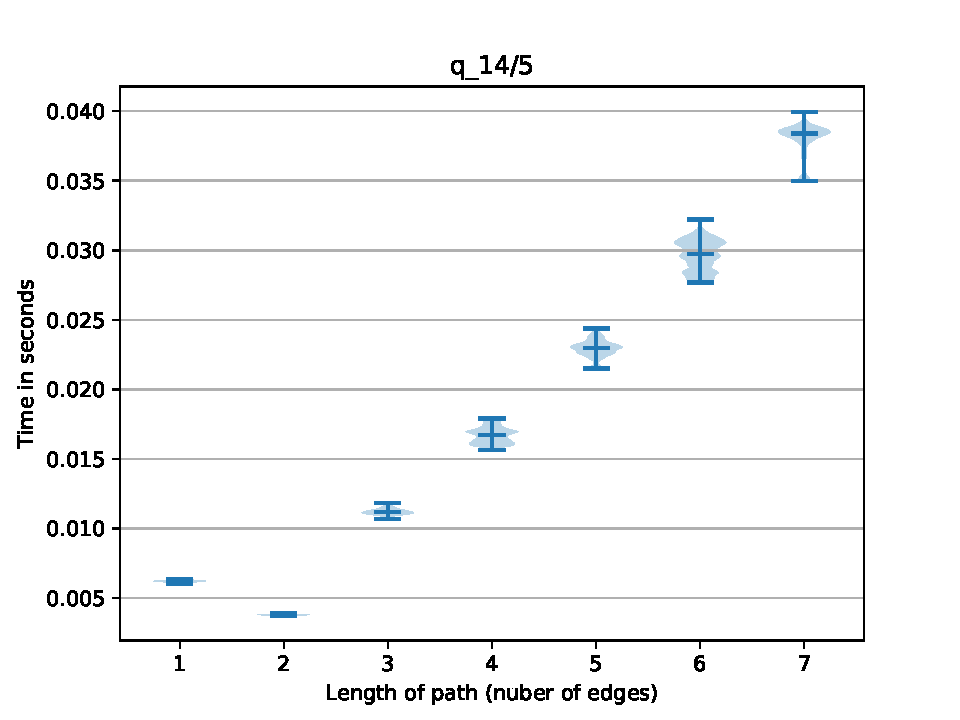
\includegraphics[width=0.48\textwidth]{data/res_graphics/q_14_5.pdf}
   \caption{Single path extraction}
\end{figure}

\subsubsection{Conclusion}

We can conclude that proposed algorithm is applicable for real-world data processing: the algorithm allows one both to solve reachability problem and to extract paths of interest in reasonable time even using na{\"i}ve implementation.  

\subsection{CFPQ Evaluation}

Comparison with matrix-based algorithm.

\subsubsection{Dataset}

Dataset for evaluation. 
It should be CFPQ\_Data\footnote{CFPQ\_Data is a dataset for CFPQ evaluation which contains both synthetic and real-world data and queries \url{https://github.com/JetBrains-Research/CFPQ\_Data}. Access date: 07.07.2020.}

\begin{table}
{
\rowcolors{2}{black!2}{black!10}
\begin{tabular}{|l|c|c|}
\hline
Graph & \#V & \#E \\
\hline
\hline 
eclass\_514en  & 120 926 & 484 646 \\
enzyme  & 358 434 & 144 9711 \\
geospecies  & 596 760 & 2 416 513 \\
go   & 1 188 340 & 4 820 728 \\
go-hierarchy & 1 780 956 & 7 228 358 \\
taxonomy & 2 308 385 & 9 369 511 \\
\hline
Aliases 1 & 6 442 630 & 24 465 430 \\
Aliases 2 & 4 834 262 & 12 366 973 \\
.... & 5 728 398 & 14 922 125 \\
\hline
\end{tabular}
}
\caption{Graphs for CFPQ evaluation}
\label{tbl:graphs_for_cfpq}
\end{table}



Same-generation queries, memory aliases.

\subsubsection{Results}

Results of evaluation.

Index creation.

{\setlength{\tabcolsep}{0.4em}
	\begin{table}
		\caption{RDFs query $G_1$ and $G_2$ (time is measured in seconds and memory is measured in megabytes)}
		\label{tbl:tableRDFQ1_appendix}
		\rowcolors{4}{black!2}{black!10}
		\small
		\begin{tabular}{| l | c | c | c | c |}
			\hline
			
			\multirow{2}{*}{Name}  & \multicolumn{2}{c|}{$G_1$} & \multicolumn{2}{c|}{$G_2$} \\
			\cline{2-5}
			                       & Tensors & RG\_CPU\textsubscript{path} & Tensors & RG\_CPU\textsubscript{path}	 \\
			\hline
			\hline
			eclass\_514en   & 0.254   & 0.195   & 0.227 & ...\\
			enzyme          & 0.035   & 0.029   & 0.036 & ...\\
			geospecies      & 0.091   & ...     & 0.001 & ...\\
			go-hierarchy    & 0.186   & 0.976   & 0.293 & ...\\
			go              & 1.676   & 1.286   & 1.368 & ...\\
			pathways        & 0.015   & 0.021   & 0.009 & ...\\
			taxonomy        & 5.366   & .....   & 3.282 & ...\\
			\hline
		\end{tabular}
	\end{table}
}


Paths extraction.

\subsubsection{Conclusion}

\section{Conclusion and future work}
In this paper, we shown how the context-free path query evaluation w.r.t. the relational and the single-path query semantics can be reduced to the calculation of matrix transitive closure. Also, we provided a formal proof of the correctness of the proposed reduction. In addition, we introduced an algorithm for computing this transitive closure, which allows us to efficiently apply GPGPU computing techniques. Finally, we shown the practical applicability of the proposed algorithm by running different implementations of our algorithm on real-world data.

We can identify several open problems for further research. In this paper we have considered only two semantics of context-free path querying but there are other important semantics, such as all-path query semantics~\cite{hellingsPathQuerying} which requires to present all paths for all triples $(A,m,n)$. Context-free path querying implemented with algorithm~\cite{GLL} can answer the queries in all-path query semantics by constructing a parse forest. It is possible to construct a parse forest for a linear input by matrix multiplication~\cite{okhotin_cyk}. Whether it is possible to generalize this approach for a graph input is an open question.

In our algorithm, we calculate the matrix transitive closure naively, but there are algorithms for the transitive closure calculation, which are asymptotically more efficient. Therefore, the question is whether it is possible to apply these algorithms for the matrix transitive closure calculation to the problem of context-free path querying.

Also, there are Boolean grammars~\cite{okhotinBoolean}, which have more expressive power than context-free grammars. Boolean path querying is an undecidable problem~\cite{hellingsRelational} but our algorithm can be trivially generalized to work on boolean grammars because parsing with boolean grammars can be expressed by matrix multiplication~\cite{okhotin_cyk}. It is not clear what a result of our algorithm applied to Boolean grammars would look like. Our hypothesis is that it would produce the upper approximation of a solution.

From a practical point of view, matrix multiplication in the main loop of the proposed algorithm may be performed on different GPGPU independently. It can help to utilize the power of multi-GPU systems and increase the performance of context-free path querying.

There is an algorithm~\cite{apspGPU} for transitive closure calculation on directed graphs which generalized to handle graph sizes inherently larger then the DRAM memory available on the GPU. Therefore, the question is whether it is possible to apply this approach to the matrix transitive closure calculation in the problem of context-free path querying.

%%
%% The next two lines define the bibliography style to be used, and
%% the bibliography file.
\bibliographystyle{ACM-Reference-Format}
\bibliography{main}

%%
%% If your work has an appendix, this is the place to put it.
%% Please note that all the content must fit within the page limits, including any appendices.
%\appendix
%
%\section{Research Methods}
% ...

\end{document}
\endinput


